In the present and in the following chapters the mechanisms of the production fast particles emitted anisotropically in the laboratory reference frame will be discussed.
According to the hypothesis that the reaction proceeds in two steps these particles are produced in the initial phase of the collision. 
Their distributions reflect the dynamics of the intranuclear cascade and the mechanisms acting in this reaction stage.

For this aim the reaction of the $p + ^{93}Nb$ at 3.5 GeV proton beam energy has been studied in details. 
The data collected by the HADES Collaboration \cite{AGAKISHIEV2012304,AgakishievPionP,
PhysRevC.90.054906,HADES_2014_Lambda_p_Nb,PhysRevLett.114.212301,
PhysRevC.94.025201,HADES_2014_Lambda_p_Nb,2018735} 
in GSI Darmstadt have been used.

In the following the HADES detection system is presented. Also the methods used for data selection, particle identification and normalization of the 
resulting distributions are described. 

The HADES detection system has been upgraded a few times in the last two decades. In this thesis the description of the experimental apparatus is given 
as it was in year 2008 when the data used here were collected. Moreover the presentation of the apparatus will be restricted only 
to these parts of detection system which were utilized for registration of the particles of interest of the current study, namely charged pions and isotopes of hydrogen.

\section{Description of experiment}

The High Acceptance Dielectron Spectrometer HADES is installed in Heavy Ions Research Laboratory 
(GSI) Darmstadt, Germany.
It was constructed in order to perform the research with proton and heavy ion beams. 
Later also the pion beams have been used.
The beams collide with the fixed targets, which can be the solid material or the liquid.
The HADES detection system permits for registration of dileptons, mesons and barions  
and creation of their energy and angular distributions. 

The general view of the HADES apparatus is shown in fig. \ref{Hades}

\begin{figure}[!h]
	% Requires \usepackage{graphicx}
	\centering\
	\includegraphics[width=120mm]{Hades}
	\caption{The schematic diagram showing HADES detector system.
	The subsystems - RICH, MDC, TOF/Tofino, Shower are composed of 6 constructionally 
	equivalent sectors. 
Such solution permits the full coverage (360$^{\circ}$) of the azimuthal angle.
The acceptance in the polar angle is assured for 18$^{\circ} < \theta < 85^{\circ}$.}
	\label{Hades}
\end{figure}

In the HADES experiment the stationary targets are used. 
This fact creates the need to extend the detection apparatus towards forward emission 
angles in the laboratory reference frame. 
HADES detection system has full symmetry along the azimuthal detection angle. 

The target system is embedded by the construction of the Ring Imaging Cherenkov detector (RICH) 
used for detection of leptons.
For registration of charged hadronic reaction products the set of Multiwire Drift Chambers (MDC) 
and the scintillating walls called TOF and Tofino are utilized. Electromagnetic calorimetry 
is performed by the electromagnetic shower detector installed at the end of detection system.
Each of the detection subsystem is composed of 6 equivalent sectors. 

%The following particles are of interest for studying the mechanism of p+Nb reactions at 3.5 GeV proton beam energy: $\pi^+$, $\pi^-$, p, d, and t. 

In the HADES experiment the registration and identification of $\pi^+$, $\pi^-$, $p$, $d$, and $t$ created in the target  
is performed by the set of Multiwire Drift Chambers (MDC) and the TOF/Tofino scintillating walls.
The momenta of particles are analyzed by magnetic field created by toroidal superconducting magnet.
The cross section of HADES apparatus used for measurement of $p+Nb$ reaction at 3.5 GeV 
is shown in fig. \ref{HadesV2}.

\begin{figure}
	% Requires \usepackage{graphicx}
	\centering\
	\includegraphics[width=120mm]{HadesV2}
	\caption{The cross section of the HADES apparatus used for  
measurement of $p+Nb$ reaction at 3.5 GeV. The most important 
detection subsystems for registration of $\pi^+$, $\pi^-$, $p$, $d$, and $t$, 
are the Multiwire Drift Chambers (MDC) and TOF/Tofino scintillating walls. 
MDC are the tracking detectors. They provide also the information about the specific 
energy losses of particles. Scintillators measure as well the energy loses 
but they work also as triggering detectors.
The momenta of particles are measured with the use of magnetic field 
of a superconducting magnet. The toroidal magnet is installed between the pairs of MDCs.}
\label{HadesV2}
\end{figure} 


\subsection{Target}

The solid target of $^{93}Nb$ has been used. 
It consisted of 12 segments installed coaxially along the beam axis.
The diameter of each segment was equal to 2.5 mm and its thickness was of 0.45 mm.
The distances between segments were equal to 4.5mm. 
Such construction of target was optimized in order to enhance the total luminosity 
for the dilepton studies. 
The positioning of the target in regard to the detection system allowed as well to register 
the primary spallation products created in each of segment of the target.
Fig. \ref{Target_reconstruction} shows the distributions of the reconstructed vertices 
of the charged pions and $H$ isotopes origin in the $p$ + $Nb$ run. The continues distribution 
of vertices covering actual target position between -60 and 0 mm is visible. 
Due to limited precision of position measurements and tracking the individual target sectors 
can not be resolved. 

\begin{figure}[!h]
    \centering
    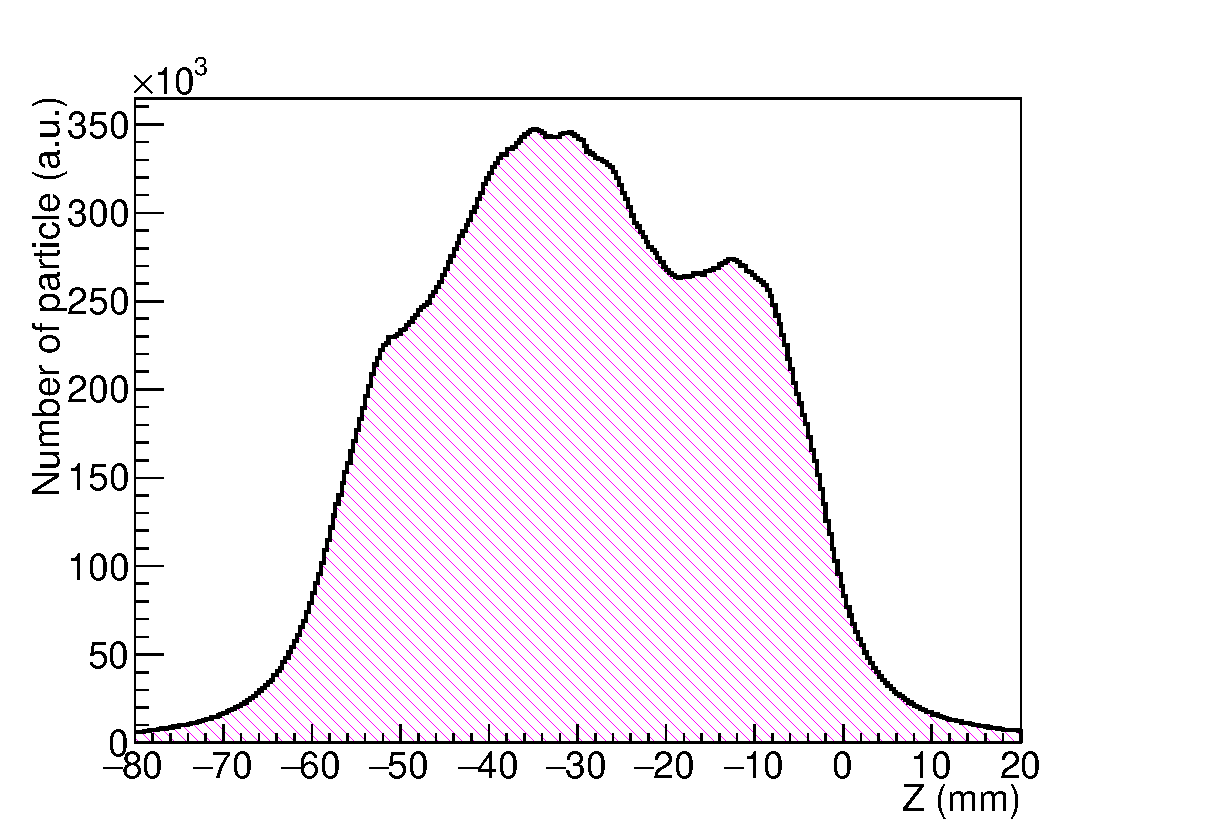
\includegraphics[width=0.9\textwidth]{Z-coordinate_target.eps}
    \caption{Distribution of track vertices of reconstructed primary charged pion and $H$ isotopes 
    during the $p$ + $Nb$ at 3.5 GeV measurement. Distributions covers the range of the segmented target
    position along the beam axis. Contributions from individual segments of target are not resolved.}
    \label{Target_reconstruction}
\end{figure}

\subsection{Multiwire Drift Chamber}
The tracking system of HADES is constructed from 24-trapezoidal Multiwire Drift Chambers (MDC). 
They are arranged symmetrically in $\phi$ angle around the beam axis. 
Each individual detection sector consists of 4 modules -  two of them are installed at front 
of the toroidal superconducting magnet and two of them behind the magnet.
The sizes of the modules increase when proceeding to the forward direction. 

The individual drift chamber (one module) is constructed of six layers. 
The angular orientation of the sense (anode) wires of each layer is different. 
The sensing wires are soldered at +40$^\circ$,  -20$^\circ$, +0$^\circ$, -0$^\circ$, +20$^\circ$ and -40$^\circ$ 
with respect to direction perpendicular to the beam axis. It is shown in fig. \ref{mdc}.   
\begin{figure}[!h]
	% Requires \usepackage{graphicx}
	\centering
	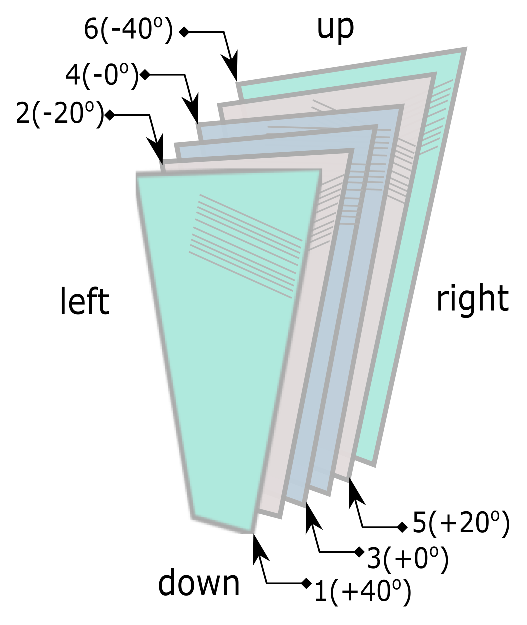
\includegraphics[width=0.45\textwidth]{mdc.eps}
	\caption{Schematic view of the sequence of six layers of each module of drift chamber 
	and the angular orientation of the sensing wires of each layer.}
	\label{mdc}
\end{figure}
The sense wires are made of tungsten which is plated with gold. 
For plane I-III the thickness of anode wires is 20 $\mu$ m whereas for the last IV plane 30 $\mu$ m.
Constant mechanical wire tension of 40 cN and 50cN, respectively, is used. 

The cathode wire are made of 80-110 $\mu m$ annealed aluminum 
(bare - plane I-III or gold plated -plane IV). 
The exact diameter of cathode wires increase with the size of chamber.
The same concerns the mechanical tension of cathode wires which varies between 150 and 180 cN.

The entrance windows of  MDCs are made from 12$\mu m$ aluminized Mylar foils.

Chambers was filled with helium-isobutane gas mixture in the proportion of 60:40. They work at atmospheric pressure.  

Position resolution of MCD system is $\le$ 100 $\mu$m in polar angle direction and $\le$ 200 $\mu$m 
in azimuthal angle direction. This permits the precise tracking and momentum reconstruction 
with the resolution of of $\delta{p}/p$ $=$ 4\%.

The effective thickness of the whole set of MDC modules is of 0.5\% of the radiation length. 
Despite of such small thickness the MDC are able to provide precise information 
about particle's energy losses. The resolution of the measured energy loss per path length, 
d$E$/d$x$, is of 7\%. The value of energy loss is measured by means of Time over Threshold 
of the detector signal \cite{Kipnis}. 
The distributions of d$E$/d$x$ vs. momentum are crucial for particle identification by means 
of their specific energy losses.



\subsection{Superconducting Magnets}

The HADES detector comprises 6 coils of superconducting magnets surrounding 
the beam axis - one coil per one sector. The coils are kept in the individual vacuum chambers. 
Each coil can generate the maximum field of 3.6 T. 
The magnetic filed of each sector was mapped with the use of a Hall probe 
and a devoted optical positioning system. 
%This mapped field also implemented into HYDRA (detector simulation tool) which is later used in efficiency calculations.    

\subsection{TOF/Tofino}

The TOF and Tofino detectors despite of their names were not used for Time-of-Flight measurement.
In the measurement of the $p+Nb$ reaction the START detector installed in vicinity of the target could not be operated.
For this reason the TOF and Tofino scintillating walls were utilized as a trigger and energy detector. 
Since they are able to provide quite precise information about energy losses of registered particles  
this advantage has been utilized in this work in order to enhance the effectiveness of particle identification.  

The TOF scintilating wall covers the $\theta$ angular range from 44$^{\circ}$ to 85$^{\circ}$. 
Each sectors comprises 8 modules of TOF detector. Each such detector consists of 8 strips of plastic scintillator. 
The thicknesses of the strip depends on their angular position and varies between 20 and 30 mm.
The time resolution of TOF scintillators is equal to 150 ps. Their position resolution is equal to 3 cm.
This results in the excellent d$E$/d$x$ resolution of the TOF detector of 4\%.  

The Tofino scintillating plastic paddles covers the gap between 18$^{\circ}$ and 45$^{\circ}$ of $\theta$ angle.
There are only 4 individual detector per one sector. 
Signals of these detectors are readout only at one side of the paddle. This results 
in the worse timing and energy resolution of Tofino walls than in case of TOF detector. 
They are equal to 420 ps and 8\% respectively.
The double hit resolution of Tofino is worse than this of TOF as well.


\subsection{Triggering}

Data Acquisition System (DAQ) in HADES experiment record the data in the event-by-event regime. 
During the collection of the data from $p+Nb$ reaction at 3.5 GeV the two independent sequences of signals triggered the (DAQ).

\begin{itemize}
\item The first trigger aimed in selection of hadronic reaction products. It required a signals of at least 3 charged particles were registered 
in TOF and/or TOFino detectors.  
\item The second trigger were constructed for identification of dileptons. The triggering condition were fulfilled if two electron signatures have been
identified in the RICH detector.
\end{itemize}

Only the first trigger were sensitive for signals from charged pions and $H$ isotopes. 
Thus, only this trigger condition is important for the goal of the present examination. 
In the following always the first type trigger is meant when the term "trigger" is recalled.

\subsection{\label{HGeant_Hydra} Software tools for tracking and simulation of detector response}

The acceptance of the total and each of the sub-detection system is simulated by the HGeant \cite{HGeant} which is a based on  GEANT3 \cite{brun1993geant} simulation package from CERN. The
full geometry, correct material budget and an accurate magnetic field map are included. Emulation of signal digitization is implemented as well.

The simulation of response of of the detection system including the trigger conditions, the tracking algorithms, energy losses, efficiencies and demanded calibrations is provided by the HYDRA framework (Hades sYstem for Data Reduction and Analysis) \cite{HYDRA}, based entirely on the C++ class package ROOT \cite{BRUN199781}. 

The initialization of apparatus geometry and the calibration parameters is possible from an Oracle database and/or from ROOT files. 

The tracking algorithms of HADES take into account the mapped magnetic field of toroidal magnet. The reconstruction of the particle trajectories in the tracking system of HADES is accomplished in several steps as described below:
\begin{enumerate}
\item The tracking algorithm demands hits in the MDC cells located in two inner modules and in two outer ones. 
The centers of the cells create a four points the space. 
Out of them the two track segments for inner and outer MDC modules are created. 
It is checked if they can be matched together within one detection sector at the so called "kick plane" as shown in figure \ref{tracking}.   
%For these four points track candidate was finally obtained through %the matching of track segments in the inner and outer drift %chambers within one sector shown in figure \ref{tracking}. 
\item For all tracks the outer track segments must match with relevant hit positions in the TOF or Tofino and the Pre-Shower detectors.
\item For identification of tracks created by electrons (not applicable in this work) the inner track segments are matched also  with rings in the RICH detector. 
\item  For such track candidate the precise hit positions within the MDC cells are calculated with the use of drift time information and 
careful calibrations of position-drift time dependence.
\item The precise 3D fitting of the predefined functions describing the particle trajectory (partially in magnetic field) is applied.  
%Using drift time information from cells the space position are %determined and a model function are fitted using this information.
\end{enumerate}

The particle momenta are determined from the bending of their trajectories inside the magnetic-field. Various algorithms 
are utilized in this respect ("kick plane", splin line, Runge-Kutta. See section 4.3 in ref \cite{agakichiev2009HADES}) . 
%Particle identification is supplemented by the information of the %particle momentum, its time of flight
%and energy loss in the TOF/TOFINO and the MDCs. Furthermore, the %correlation with a reconstructed ring
%in the RICH detector and a detected electron shower in the %Pre-Shower detector provide an efficient lepton
%identification.

\begin{figure}[!h]
	% Requires \usepackage{graphicx}
	\centering
	\includegraphics[width=0.65\textwidth]{tracking}
	\caption{Schematic view of track reconstruction using MDC detectors. Only one layer of the MDC detector is shown to simplifying the diagram.  }
	\label{tracking}
\end{figure}
 
 
The Ring Imaging Cherenkov (RICH) detectors and the Pre-shower detectors shown in fig. ref{HadesV2} have not been used for the current studies, 
thus their description is avoided in this thesis. The reader interested in these subsystems is asked to referee to \cite{agakichiev2009HADES}.

\section{\label{Analysis} Methodology of data analysis}

For the examinations of mechanisms acting during the nuclear spallation and for the developments of accurate theoretical models  
the precise and possibly most exclusive observable are needed.
The simple observable like particle multiplicities or the total production cross section are less sensitive for details 
of interplaying mechanisms than e.g. the angular or energy distributions of the reaction products or their coincidences.

Of course, the most demanded would be the experiment allowing for complete registration of all reaction products 
in 4$\pi$ geometry and in the whole kinematic range. Unfortunately such experiments are not planned. 
Thus, taking advantage of the broad acceptance of HADES apparatus and of its magnetic spectrometer 
it was decided that the double differential cross sections ($d^2\sigma/d\Omega dE$) will be derived as a 
first portion of spallation data delivered by HADES experiment. 

Three significant difficulties have been encountered when the selection and particle identification (PID)  
of primary spallation products from $p+Nb$ run at 3.5 $GeV$ reaction have been performed.
\begin{enumerate}
	\item At least 3 charged particles are demanded in the TOF/Tofino walls in order to fulfill the trigger condition. 
	This fact implicated that the purely single distribution spectra were not registered. 
	\item The origin of triggering particles was disregarded by the trigger system. 
	It means that both the reaction products originating from the target 
	as well as the secondary particles created in the parts of apparatus could contribute to the trigger.
	\item Due to missing START detector the Time of Flight (TOF) measurement could not be done. 
	Thus, the PID based on the $\beta$ value of particles was significantly reduced. 
    To some extent the particle TOF could be estimated by comparison to the of timing information 
    of the identified fastest particles contributing to the trigger. But as long as the single distribution 
    of reaction products are of interest the coincidences with other particles have to be disregarded.
    In the present analysis the reconstructed TOF values were used only for preselection of data. 
    The lack of actual TOF information significantly reduced the identification energy ranges for $\pi{^+}$, $d$ and $t$.	
\end{enumerate}

Such problems are not present during identification of leptonic or hadronic products 
produced with much smaller cross sections which are of main interest of the HADES collaboration.  



%\subsection{\label{PID} Particle identification and background subtraction}
\subsection{\label{PID} Particle identification}
\begin{figure}[!h]
		% Requires \usepackage{graphicx}
		\centering
		\includegraphics[width=0.90\textwidth]{MassCut.png}
		\caption{{\it Left panel: the mass vs. momentum distribution of registered particles. The mass is calculated from the reconstructed TOF value. 
		(\it Right panel:} projection of distribution of left panel onto mass axis.) }
		\label{MassCuts}
	\end{figure}
	\begin{figure}[!h]
		% Requires \usepackage{graphicx}
		\centering
		\includegraphics[width=0.95\textwidth]{projection.png}
		\caption{{\it Left panel:} The $dE/dx$ vs. $momentum$ distributions for protons registered in MDC. The distribution is created with the use of predefined
		mass cuts (see above). Distribution is divided into bins of the 25 MeV/c width. Slot for 725 - 750 MeV/c is marked with the red color vertical strip.
		{\it Right panel:} The projection of proton distribution of 725 - 750 MeV/c momentum bin onto the $dE/dx$ axis. The superimposed distribution given 
		in red color is the asymmetric Gaussian function (cf. formula \ref{aGauss}). 
		}
		\label{Projec}
	\end{figure}
As mentioned above the identification technique used in this thesis utilizes the momentum dependency of the specific energy loss 
per particle path length in the detector, $dE/dx$.
However, only for the initial - most general definition of identification cuts the 
mass dependence (calculated from reconstructed TOF) on momentum were utilized.

The scheme of PID was as follows:

\begin{enumerate}
	\item The mass distribution of the registered particles was calculated knowing theirs reconstructed TOF.  
	The results in the function of particle momentum is shown in figure \ref{MassCuts} - left panel. 
    \begin{figure}[!h]
   	% Requires \usepackage{graphicx}
   	\centering
   	\includegraphics[width=0.95\textwidth]{MDC_CUTS.png}
   	\caption{The scatter plot of $dE/dx$ vs. $momentum$ for $p$, $d$, $t$ and $\pi^+$ registered in MDC. The identification cuts of three widths 
   	(described above) are superimposed. 
    }
   	\label{MDCcut}
   \end{figure}
	\item The mass vs. momentum distributions is projected onto mass axis and initial slots of mass cuts are defined. 
	The results are shown in \ref{MassCuts} - right panel. 
	\item Such defined mass cuts are used for creation of $dE/dx$ vs. $momentum$ distributions for $p$, $d$, $t$, $\pi^+$ registered in MDC. 
	The example of such scatter plot for protons is presented in fig. \ref{Projec} - left panel.
    \item The dE/dx vs. momentum distributions are divided into 25 MeV/c momentum bins as indicated in fig. \ref{Projec} - left panel.
    \item Part of distribution comprised in each 25 MeV/c momentum bin is projected onto the $dE/dx$ axis 
    (cf. fig. \ref{Projec} - right panel where the example for protons of the momenta 725 - 750 MeV/c is given).
    
   \item Asymmetric Gaussian function of formula \ref{aGauss} is fitted for resulting distribution of every 25 MeV/c momentum bin. Example of fitted function 
   for protons of the momenta between 725- and 750 MeV/c is superimposed on the particle distribution in fig. \ref{Projec} - right panel. 
   Formula for asymmetric Gaussian function:
    \begin{equation}
   	f_g(x)=\begin{cases}
   		\frac{1}{\sigma_l\sqrt{2\pi}}e^{-\frac{1}{2}\left(\frac{x-\mu}{\sigma_l}\right)^2}&\mu\le0\\
   		\frac{1}{\sigma_r\sqrt{2\pi}}e^{-\frac{1}{2}\left(\frac{x-\mu}{\sigma_r}\right)^2}&\mu>0
   	\end{cases}
   \label{aGauss}
   \end{equation}
   
   \begin{figure}[!h]
   	% Requires \usepackage{graphicx}
   	\centering
   	\includegraphics[width=0.95\textwidth]{TOF_CUTS.png}
   	\caption{Description is same as fig. \ref{MDCcut} but for TOF detector. 
    }
   	\label{TOFcut}
   \end{figure}
 

   \begin{figure}[!h]
   	% Requires \usepackage{graphicx}
   	\centering
   	\includegraphics[width=0.95\textwidth]{TOFino_CUTS.png}
   	\caption{Description is same as fig. \ref{MDCcut} but for TOFino detector.
    }
   	\label{TOFinocut}
   \end{figure}
   \item The $\mu$ and $\sigma$ of the asymmetric Gaussian fit are used to determine the various width of the MDC cuts. 
   The widths of cuts are given by calculated values of [$\mu - \sigma_i \times m$, $\mu + \sigma_i \times m$]) 
   where $m$ takes values of 0.6, 0.8, 1.0, 1.2 and 1.5. The examples of MDC $dE/dx$ vs. $momentum$ distribution of $p$, $d$, $t$, $\pi^+$
   with superimposed MDC cuts of three different widths are shown in fig. \ref{MDCcut}. 
   Using of various cut widths is needed in order to estimate the systematic uncertainty of the PID method. This point will be recalled when
   the systematic error components will be discussed (see chapter \ref{Uncertainties}).
   
  \item The particle distributions selected with the use of MDC cuts are further used to create the $dE/dx$ vs. $momentum$ distributions 
  and the identification cuts but for reaction products registered in TOF/Tofino detectors.
  For this aim the points 3 - 7 of the analysis scheme are repeated. Multiplication factors $m$ 
  for TOF/Tofino cuts are equal to 0.6, 0.8, 1.0, 1.2, 1.5 and 1.8. 
   These spectra are used for derivation of both the distributions containing the 
  "signal" of the searched for cross section as well as for identification of the background component.Examples of the $dE/dx$ vs. $momentum$ distributions for TOF and Tofino detectors are shown 
  in fig. \ref{TOFcut} and fig. \ref{TOFinocut}. 
    
  \end{enumerate}
  
  In this three-level approach (after demanded smoothing) the most precise 2D identification cuts for $dE/dx$ - $momentum$ distributions are defined.
  Finally they are applied for the row data distributions (disregarding the initial mass cut) in order to identify the reaction products of interest
  unbiased with the reconstructed TOF value. 

  The separation of negatively charged pions from other reaction products is provided by their opposite deflections in the magnetic field. 
  For them the definition of identification cuts is not needed. The contamination of the $\pi^{-}$ spectra with the $K^{-}$ is insignificant 
  and for this reason neglected in this analysis.


\subsection{\label{Back_sub} Signal and background identification}

In the current work the emphasis is put on the kinetic energy and angular dependence 
of the production cross section.
(For now on when the term "energy" is used always the kinetic energy of the emitted particle is meant).   
In order to study the angular dependence of cross section 
the $dE/dx$ - $Energy$ distribution of particles detected in TOF/Tofino detectors
are prepared for the selected emission angles between 
20$^{\circ}$ and 85$^{\circ}$ with the step of 5$^{\circ}$.
The identification 2D cuts of different widths as defined above are applied. The example of identification cuts of three different width $\mu$ for deuterons detected at the emission angle of  ??? is shown in fig.  \ref{deuteron_cuts_tofino}. \\
\begin{figure}[!h]
    \centering
    \includegraphics[width=0.95\textwidth]{Deuteron_TofinoCuts.png}
    \caption{Example o the identification cuts applied for selection of deuterons detected at $\theta$ laboratory angle of ??. Three different width $\mu$ of the cuts are shown.}
    \label{deuteron_cuts_tofino}
\end{figure}
The resulting distributions (which should contain mainly identified reaction products)  
are bin-by-bin projected onto $dE/dx$. The momentum bin is equal to 25 MeV.

In effect the one dimensional distributions of energy losses in TOF or Tofino detectors are obtained.
They comprise the component of the searched for particle superimposed on the background formed by the 
misidentified particles of the lower or higher mass. Fig. \ref{backg} presents examples of such distributions   
for $p$, $d$, $t$ and $\pi^+$  registered at $\theta$ = 25$^{\circ}$ and for various energy bins.
They are done as well for selected widths of identification cuts.

It is well visible that the particle identification scheme described above has limited strength. 
The selected distributions of reaction products of interest  
are still superimposed on the distributions of misidentified particles, which form the background. 

In order to calculate both the signal and background components 
of the distributions the fitting of the appropriate functions is performed. 

The functions which approximate the shapes both of the signals as well as 
the background distributions in principle should be the Landau functions. 
Landau functions describe the best the distributions of energy losses 
in solids ad in the gasses of due to individual interactions of charged particles 
with the atoms or molecules of the medium in the studied hire energy range. 
However in the case of this analysis it turned out that both the signal and background 
distributions do do follow the Landau function. 
It is due to the fact that the multi-step cuts applied to the raw data caused 
the truncations of the original experimental distributions of events.  

Thus, in described here method the signal is fitted always as an asymmetric Gaussian. 
(In fig. \ref{backg} the fitted functions 
of the signal components are given with green color and superimposed on the experimental distribution). 
It is tried to fit the signal distribution in the range where the signal component 
is clearly separated.

For the protons and pions (in the latter case for the limited energy range) 
the components of "signal" are dominant. 
The background is small and easy to identify. 
Its component can be approximated by the linear function fitted 
to the both sides of the "signal" distribution. 
In fig. \ref{backg} the fitted contributions of background are given with red color.

Much worse signal to background ratio is obtained for deuterons. 
However still the component formed by deuterons is clearly 
separated from the component originating from protons. The background is fitted as an exponent.

The most difficult was to separate the tritons from background components originating 
from other species mainly from deuterons. In fig. \ref{backg} (c) the signals from tritons is small 
in comparison to well visible peaks of $p$ and $d$.

\begin{figure}[!h]
		\centering
		\includegraphics[width=0.95\textwidth]{allBackground.eps}
		\caption{The $dE/dx$ distribution for $p$, $d$, $t$ and $\pi^+$ registered in Tofino detectors 
                at laboratory $\theta$ angle of 25$^{\circ}$. Examples show distributions for various energy bins 
                and selected with various widths of identification cuts. 
                These spectra provide the information both about the "signal" component of the cross section 
                as well as the background of misidentified particles. The fitted distributions of signal (green color) and 
                background (red color) are superimposed.}
		\label{backg}
\end{figure}  


Various efforts to separate the net component of triton from the dominant background were undertaken. 
The most effective one occurred to be ......

\vspace{5cm}
needs to be described .... \\


The separations of individual components of $dE/dx$ distributions for positively charged reaction product 
varies with the energy of particles. It is better for the lower energies and deteriorates when particle energy increase.
The distributions of specific energy losses gets closer each to other with the energy rise.

At some energy the signal to background ratio is so unfavorable the identified 
signal component is charged with too high uncertainty.
In this thesis it was selected that the signal is separated from background 
if for the applied width of cut the signal to background ration is greater than 50 \%. (???) 

Fig. \ref{sig_back_separation} shows the example of experimental PID distributions for .... and for .... energy bins. 
In this case the maximal energy when the signal distribution is separated from the background is equal to ... .

 \begin{figure}
   	% Requires \usepackage{graphicx}
   	\centering
%   	\includegraphics[width=0.95\textwidth]{sif_back_separation_....png}
   	\caption{PID distributions for .... . Example for ... energy bin of ..... Separation of signal from background is possible
   	below energy of .... . Above this value the signal to background ratio gets lower than 50 \%.
    }
   	\label{sig_back_separation}
   \end{figure} 


The net value of the signal component for the given energy bin is calculated by subtracting the area of the fitted background function from the area of the 
fitted signal functions. It is important to stress that the subtraction is done only in the selected limits, which are narrower than the range 
of fitted signal distribution. This limits are related to the  mean value, $\mu$, and the standard deviation, $\sigma$, of the fitted Gaussian 
function. They are calculated as:  
[$\mu$ - $\sigma$ $\cdot$ $m$, $\mu$ + $\sigma$ $\cdot$ $m$] where $m$ = 0.6, 0.8, 1.0, 1.2, 1.5, 1.8 

The amount of events contributing to the searched for specific cross section 
at given laboratory emission angle $\theta$ and for given energy bin 
is calculated as an average of the values obtained 
for all applied multiplication factor $m$.  

The PID/background identification were not necessary for well identified by the HADES apparatus itself the $\pi^+$ distribution. 


% %For this reason the PID and background 
% %subtraction will be considered together. 
% To determine the background and to subtract it from the distribution of reaction products of interest the following methods have been applied:
% \begin{itemize}
% 
% 	\item The distributions of TOF/Tofino 
% 	
% 	First MDC cuts are applied which is determined in the above 
% 	text then again TOF/TOFino detector dE/dx vs momentum distribution 
% 	for angles (20,25,30,...$85^o$) is plotted. 
% 	The corresponding width of cuts(for m = 0.6, 0.8, 1.0, 1.2, 1.5, 1.8) are applied 
% 	to determining the background in each width of TOF/TOFino cuts.
% 
% 	\item After plotting a distribution for a particular angle and with of cuts for TOF/TOFino detectors. 
% 	The distributions of selected particles (within the cuts) after their projections to $dE/dx$ axis 
% 	the fits of signal and background distributions have been performed for a given in range 
% 	of ($\mu-\sigma_l*m , \mu+\sigma_r*m$) where m = 0.6, 0.8, 1.0, 1.2, 1.5, 1.8 
% 	and sigma values are taken from earlier fits. For example background calculation for p, d, t, and $\pi^+$ 
% 	at angle $\theta=25$ and width $\mu \pm \sigma_{l/r}\times1.5$ is shown in figure \ref{backg}.
% 	\begin{figure}
% 		\centering
% 		\includegraphics[width=0.95\textwidth]{PidBackground.png}
% 		\caption{Background}
% 		\label{backg}
% 	\end{figure}  
% \end{itemize}


\subsection{\label{Eff_corr} Efficiency and acceptance corrections}
Proper calculation of geometrical acceptance and the efficiency of
the overall detection and acquisition system (DAQ) is crucial for
correct calculation of absolute values of studied here cross
sections. These quantities remain in complicated dependence on
detection geometry, composition of the detection system, types of
primary particle and their energy- and angular distributions, the
yields of secondary particles and their distributions, the
efficiencies of individual detectors, condition of trigger, death
time of DAQ.
The calculation of cross section corrections caused by geometrical
restriction and finite efficiencies can be done only with the help
of software tools explained already in subsection 3.1.6. The exact
geometry of the apparatus and the response of the detectors to the
irradiation is implemented into the HGeant package \cite{HGeant}. HGeant is
based on the Geant3 toolkit \cite{brun1993geant}.

The actual conditions present during the data taking are considered by the HYDRA framework \cite{HYDRA}. 
This package contains as well all needed calibrations, tracking 
tools, electronic response to primary particles and emulation of trigger logic (cf. \ref{HGeant_Hydra}). 

In principle the acceptance and efficiency of the detection system has to be calculated as a ratio of two distributions:
\begin{enumerate}
\item the so called "ideal" distribution - it is obtained by simulation of well known and dominant processes 
with assumption that the 4$\pi$ detection geometry is available and the overall efficiency 
of the detection system is equal to 100 \%.  
\item the "real" distribution - obtained by simulation of the same processes but including the geometrical restriction 
and finite efficiencies of all components of HADES detection system. These restrictions are included 
to the HGeant and Hydra software.
\end{enumerate}

Of course the product of efficiency and acceptance,
(Efficiency x Acceptance - $EA$), is dependent on the energy, emission angle and the kind of the emitted particle. It is given by the formula:\\
 \ \\
\begin{equation}
\label{EA_eq}
    EA(Z, A, E, \theta) = \frac{real(Z, A, E, \theta)}{ideal(Z, A, E, \theta)}
\end{equation}

 \ \\
where the $Z$, $A$ are the atomic and mass number of particle of energy $E$ emitted at laboratory angle $\theta$.

Both the "ideal" as "real" distributions are simulated as a scatter plots $\theta$ vs. $Energy$. They have to be divided bin by bin for reasonable selected angular and energy bin widths.
Ideal, real and resulting $EA$ distributions for obtained for combination of INCL++ + HGeant + Hydra frameworks (see below) 
are presented in fig. \ref{EA_INCL}. 

For the specific case of the single spectra of spallation reaction studied in this work, 
it was needed to test if $EA$ calculated in such a way is independent of the conditions applied in simulations.

In the first step of $EA$ calculation it was checked if 
this method is robust against the kind of event generator used for simulations 
of ideal and real distributions.

The simulations were done using the event generator which simulate the isotropic emission of protons of the energy sampled from the range [0,3500] MeV into the full solid angle. It turned out that when the initial multiplicity of protons is equal to 8 
the resulting EA is smaller than when the multiplicity of generated protons is equal to 16.
Examples of such calculation of $EA$ for registration  of protons at the laboratory emission angle $\theta$ = 37.5$^{\circ}$ $\pm$ 1.5$^{\circ}$ are shown in fig. \ref{IsoEff}. $EA$ values obtained when multiplicity of initial protons are equal to 16 (fig. \ref{IsoEff} (b)) are larger by $\sim$9\% from those for isotropic event generation with multiplicity of 8 (fig. \ref{IsoEff} (a)).  

    \begin{figure}
    \centering
	\begin{subfigure}[b]{0.45\textwidth}
		\includegraphics[width=\textwidth]{EffIsot8.png}
		\caption{\label{IsoEff8} Mutiplicity 8.}
	\end{subfigure}
	\begin{subfigure}[b]{0.45\textwidth}
		\includegraphics[width=\textwidth] {EffIsot16.png}
		\caption{\label{IsoEff16} Mutiplicity 16.}
	\end{subfigure}
	\caption{\label{IsoEff} Product of Efficiency and Acceptance,  $EA$, for detection of protons at laboratory angle of $\theta$ = 36$^\circ$-39$^\circ$. Event generator simulating the emission of protons with multiplicity 8 (a) and 16 (b) into the full solid angle were used. Kinetic energies of generated protons were ranging from 0 to 3.5 GeV. For details see text.}
\end{figure}

This findings indicated that the calculation of $EA$ might 
be biased by improper selection of event generator. The reliable value of $EA$ must be calculated with the use of the event generator
which approximates sufficiently precise at least the dominant production and emission processes 
in the target. This include both the types and yields of particles emitted from the target as well as their energy0 and angular distributions.

For these reason it was decide to use the INCL++ model. Is was many times confirmed that this model reproduce the multiplicities, energy and angular distributions of dominant spallation products with the precision of factor about 2, what was anyway the best achievement among the spallation reaction models \cite{INCLMancusi2014,UrQMDBASS1998,UrQMDBleicher1999}.
 
    \begin{figure}
	% Requires \usepackage{graphicx}
	\centering
	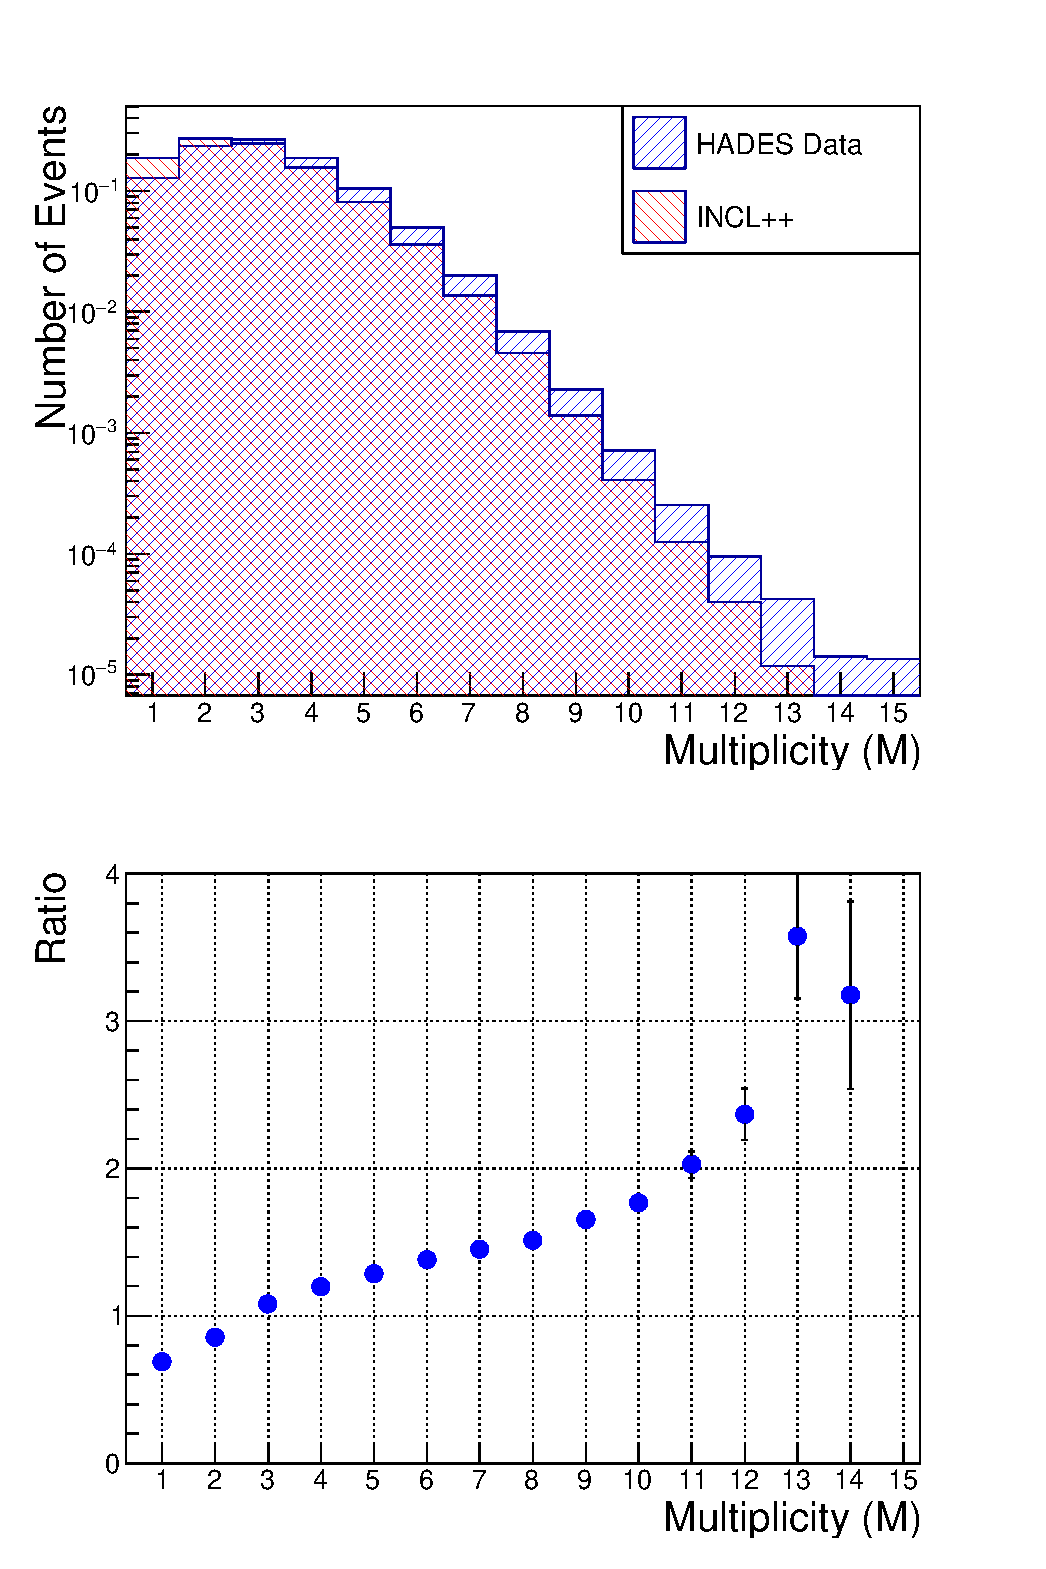
\includegraphics[width=0.6\textwidth]{MultINCL}
	\caption{Upper panel: multiplicity distribution of primary particles obtained by simulations with the use of HGeant + Hydra software and the INCL++ model as a event generator.
	The theoretical distribution is compared to the experimental one registered in HADES with the use of the same software tools used for tracking and EA corrections. 
	Both distributions are normalized to the same total number of events. Lower panel: ratio between the experimental and simulated distributions.}
	\label{MultINCL}
    \end{figure}

The correctness of the INCL++ model used as an event generator for calculation of overall $EA$ values in the present studies is confirmed by the good agreement of experimental and simulated multiplicities of detected particles for $p$ + $Nb$ reaction measured at HADES. It is shown of fig. \ref{MultINCL}.  

The experimental distribution there comprises only those particles 
which tracks could be reconstructed back to the target position.  
It means that only primary particles produced in the target contribute to the multiplicity distribution. The secondary particles, which contributed to the trigger (trigger condition demands at least 3 charged particles in the TOF/Tofino 
scintillating walls) are suppressed. For this reason experimental distribution contains the contribution from multiplicity equal 1 and 2. 

Simulated distribution (marked in fig. \ref{MultINCL} as "INCL++")
is obtained with the use of the same HGeant and Hydra environment and parameters as it was used for creation of experimental distribution of multiplicity in $p$ + $Nb$ reaction ( !!!! is it true ? Secondaries are there !!!). In simulations the energy of bombarding protons used for generating the particles entering the detection system was set the same as energy of beam protons, i.e. 3.5 GeV.  

For the most dominant multiplicities of events (between 1 and 7) 
the ratios of experimental/simulated distributions varies between 0.7 and 1.4. It is a proof that an INCL++ is an sufficiently realistic event generator for the studied reaction. Experimental conditions can be reasonably well reproduced by INLC++ + HGeant + Hydra combined frameworks. $EA$ values calculated with use of these 
tools is reliable.  

The problem of possible bias of the calculated efficiency for registration of single spectra in HADES by the trigger conditions required coincidences of at least 3 charged particles will be addressed in subchapter \ref{eff}.   

The ideal and real distribution were simulated for each of reaction products studied in this thesis and the scatter plots of $\theta$ vs. $Energy$ were created. In order to assure the smooth dependence but also the sufficient resolution the binning of the both axes 
has been optimized. Finally the width of energy bin was selected as 
... MeV and the bin of angle was ... degrees.

The examples of the $ideal$ and $real$ 2D distribution for ... 
as well as the resulting EA distribution calculated for each energy-angle bin according to formula \ref{EA_eq} are shown 
in fig. \ref{EA_INCL} a, b and c, respectively.

    \begin{figure}
    \centering
	\begin{subfigure}[a]{0.45\textwidth}
%		\includegraphics[width=\textwidth]{EA_ideal.png}
		\caption{\label{EAideal1} $ideal$ distribution }
	\end{subfigure}
	\begin{subfigure}[b]{0.45\textwidth}
%		\includegraphics[width=\textwidth] {EA_real.png}
		\caption{\label{EAreal2} $real$ distribution}
		\end{subfigure}
	\begin{subfigure}[c]{0.45\textwidth}
%		\includegraphics[width=\textwidth] {EA.png}
		\caption{\label{EAreal3} EA distribution}
		\end{subfigure}		
	\caption{\label{EA_INCL} FIGURE IS MISSING HERE 
	Product of Efficiency and Acceptance,  $EA$. 
	(a) (b) (c) .... 
	    }
\end{figure}

In order to obtain the energy dependence of efficiency 
for the selected emission angle the demanded angular 
slit is defined and the two dimensional EA distribution 
is projected onto energy axis. Such example is given in fig. \ref{Deuteron_efficiency} where 
product of overall efficiency of the system and its geometrical acceptance is shown for detection of single distribution of deuterons emitted from target at 43.5$\pm$1.5$^{\circ}$ laboratory $\theta$ angle. The EA values calculated without the PID cuts applied for $real$ distribution is given with red dots whereas the 
EA distribution reduced due to selection of fraction o experimental distributions defined within the PID cut is shown by blue dots. As described in \ref{{PID}} for assessment of systematic uncertainty calculation of cross section with the use of various widths of PID cuts were used. The width of PID cuts applied for simulations 
were always the same as those defined for experimental distributions. In case of reduced EA distribution 
of fig. \ref{Deuteron_efficiency} the width of the PID cut was equal to 0.8 $\sigma$.

   \begin{figure}[!h]
        \centering
        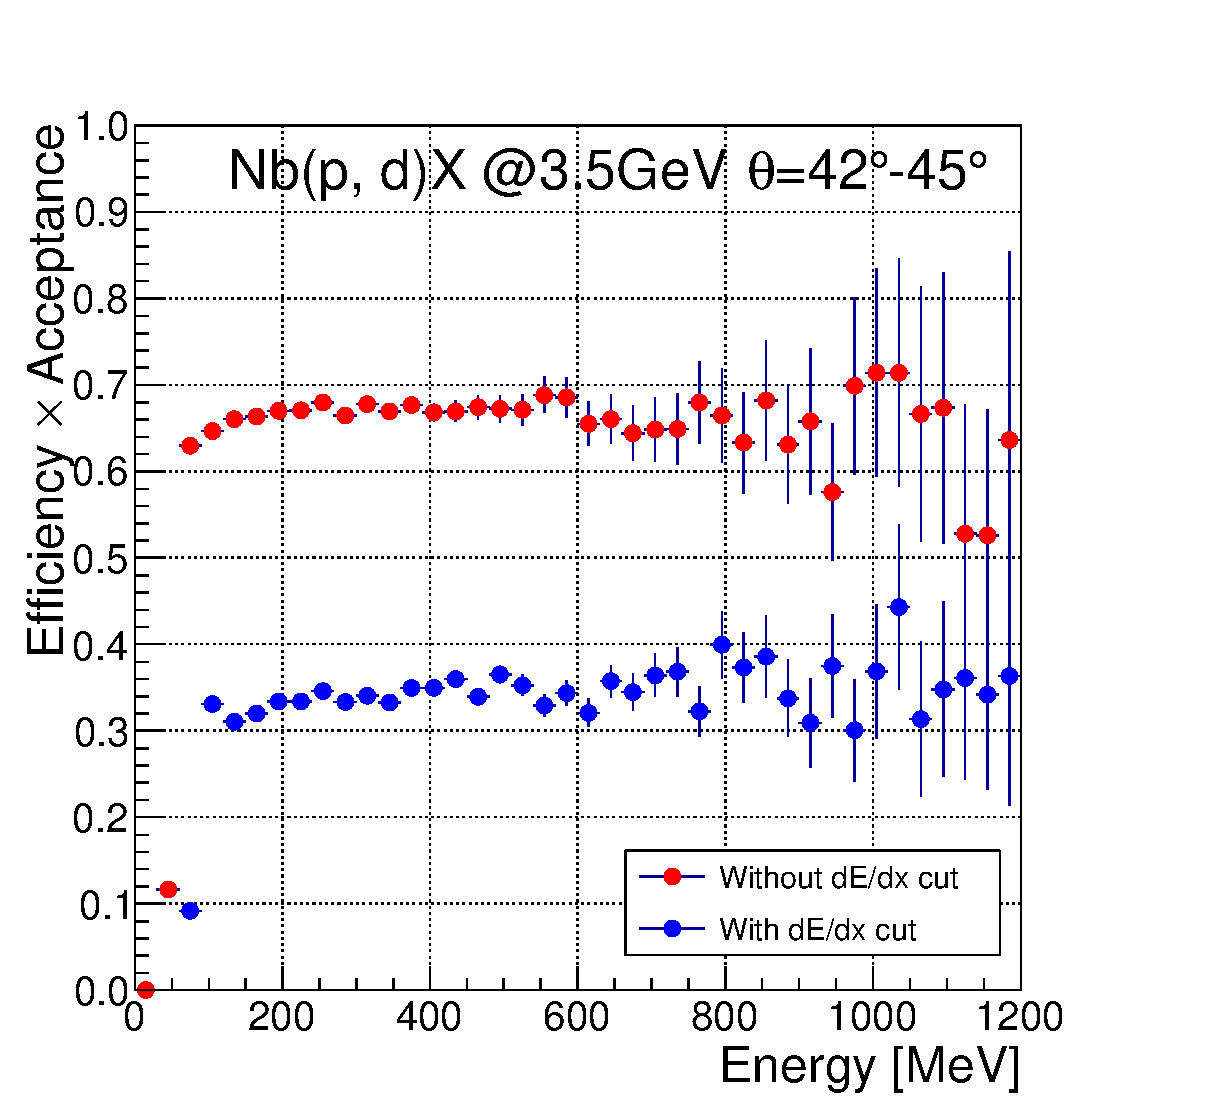
\includegraphics[width=0.65\textwidth]{DeuteronEfficiency.eps}
        \caption{Example of HADES efficiency for registration of deuterons at $42^\circ < \theta< 45^\circ$
        laboratory angle. The red dots represent the efficiency obtained when the PID cuts were not
        used whereas the blue dots show the final energy dependence
        of efficiency used for correction of absolute cross section. In this case the PID cut of the width equal to 0.8 $\sigma$ 
        is applied to the ”real” distributions of deuterons.}
        \label{Deuteron_efficiency}
    \end{figure}
  

The flow chart showing in details the steps of calculation of the EA distributions and optimization of event generator is shown in appendix (cf. \ref{App1}). 


% In order to absolute normalization of the cross-section the overall efficiencies of different particles i.e p, d, t, $\pi^-$ and $\pi+$ was determined. In the case of the current study, it is a product of detection efficiencies of various components of the HADES system, the effectiveness of the data acquisition system, the trigger conditions and the distributions of secondary particles created in the HADES setup and contributing to the triggering of event. The total efficiency is depended on energy, theta and type of particle.


% \begin{figure}
% 	% Requires \usepackage{graphicx}
% 	\centering\
% 	\includegraphics[width=0.95\textwidth]{INCLEff}
% 	\caption{The scatter plot of dE/dx (MDC) vs. momentum for protons. The cut obtained from 
% 		the asymmetric Gaussian fits is shown. The theoretical calculation of energy loss according to Bethe-Bloch formula is shown as well with the red line.}
% 	\label{INCLEff}
% \end{figure}
% \begin{figure}
% 	% Requires \usepackage{graphicx}
% 	\centering\
% 	\includegraphics[scale=0.6]{Efficiency}
% 	\caption{The scatter plot of dE/dx (MDC) vs. momentum for protons. The cut obtained from 
% 		the asymmetric Gaussian fits is shown. The theoretical calculation of energy loss according to Bethe-Bloch formula is shown as well with the red line.}
% 	\label{Eff}
% \end{figure}
% \begin{figure}
% 	% Requires \usepackage{graphicx}
% 	\centering\
% 	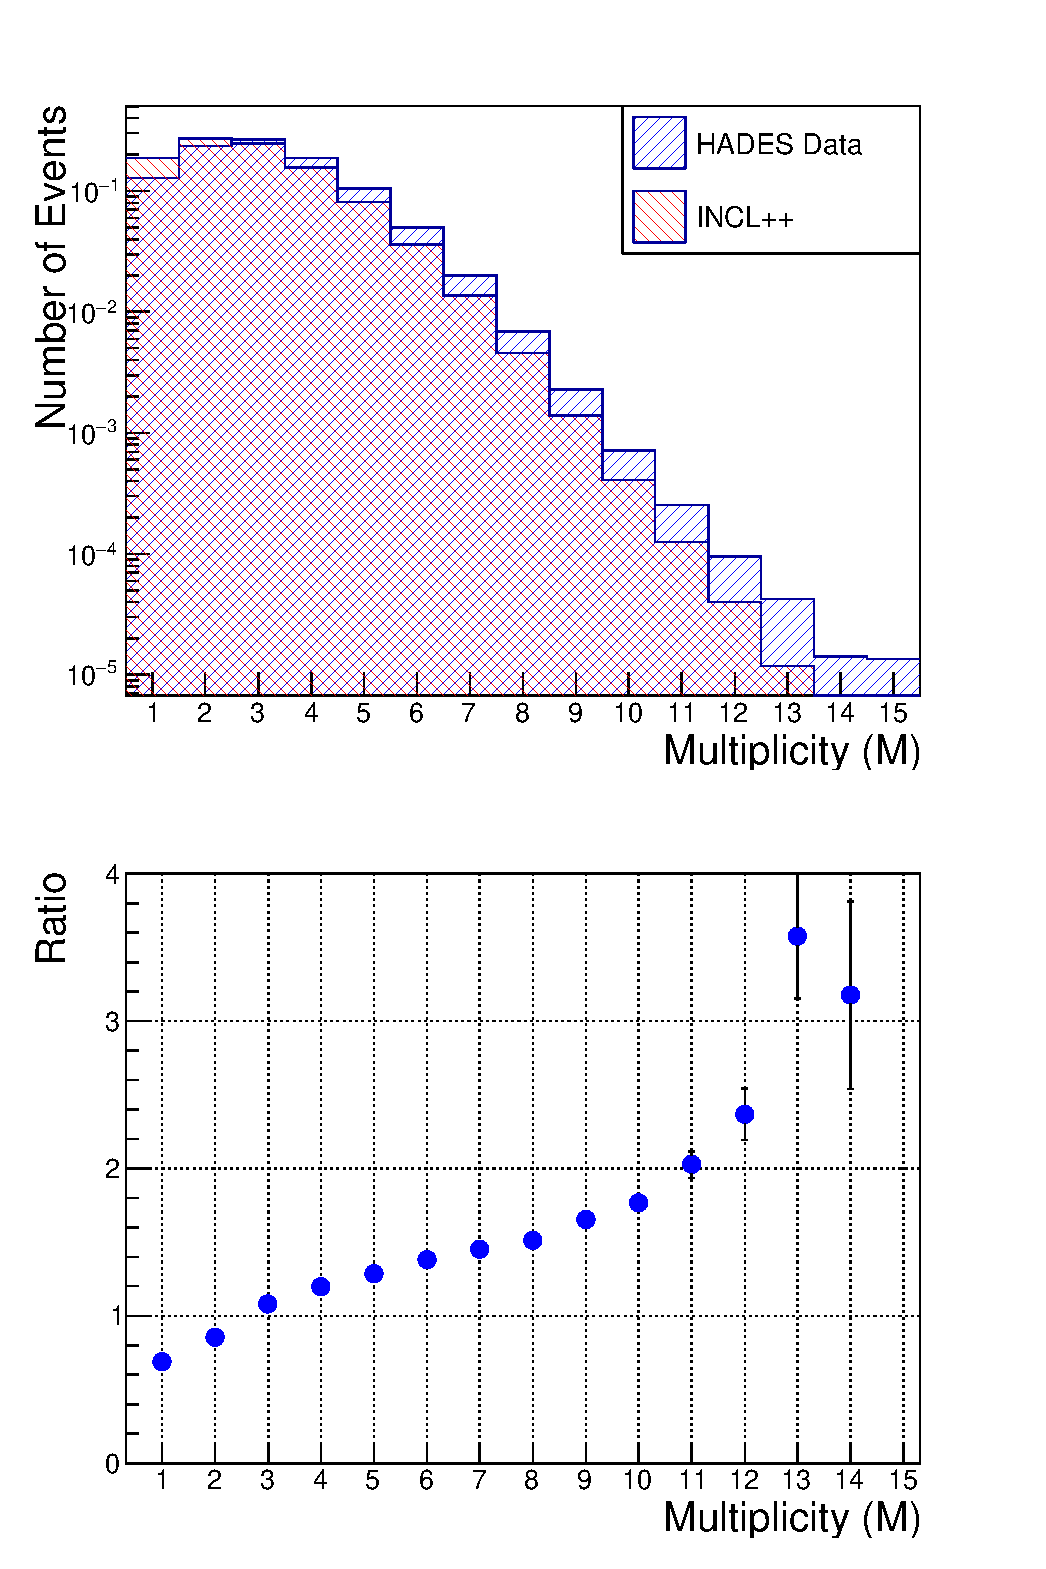
\includegraphics[width=0.95\textwidth]{MultINCL}
% 	\caption{In this figure various parts of RICH detector is shown }
% 	\label{MultINCL}
% \end{figure}
% \begin{figure}
% 	% Requires \usepackage{graphicx}
% 	\centering\
% 	\includegraphics[width=0.95\textwidth]{Efficiency2}
% 	\caption{The scatter plot of dE/dx (MDC) vs. momentum for protons. The cut obtained from 
% 		the asymmetric Gaussian fits is shown. The theoretical calculation of energy loss according to Bethe-Bloch formula is shown as well with the red line.}
% 	\label{Eff2}
% \end{figure}
% \begin{figure}
% 	% Requires \usepackage{graphicx}
% 	\centering\
% 	\includegraphics[width=0.95\textwidth]{runningAverage}
% 	\caption{The scatter plot of dE/dx (MDC) vs. momentum for protons. The cut obtained from 
% 		the asymmetric Gaussian fits is shown. The theoretical calculation of energy loss according to Bethe-Bloch formula is shown as well with the red line.}
% 	\label{RA}
% \end{figure}




\subsection{\label{Uncertainties} Experimental uncertainties} 
 
The broad acceptance and overall high luminosity for the experiment when $p + Nb$ at 3.5 GeV reaction was measured 
provided huge statistics of collected events. 
Thus, the statistical error of the measurement is insignificant and will not be considered in this work. 
 
The components of systematic uncertainty are discussed below. They origin from:
\begin{itemize}
	\item misidentification of signal and background particles 
	due to imperfectness of PID cuts, the limited quality of fits for the signal and background distributions 
	and the uncertainty of background dispersion; 
	\item calculations of efficiency and acceptance of the apparatus
	%(applied event generator, limited statistics of simulations, bin-to-bin dispersion of correction factors);
	\item deviations in the performance  of individual sectors of HADES detection system;
	\item uncertainty of absolute normalization of the data used in HADES experiment.  
\end{itemize}

The lasts component of the systematic error is constant and equal to 15\%.
This value is adopted from the data analysis performed in the HADES collaboration already 
in the past with the use of the same data but for other reaction products \cite{AgakishievPionP,Tlusty, Lorentz_PhD}.
In that case the comparison of the HADES results to the pion data measured by HARP-CDP collaboration \cite{Tlusty} 
were done.

The total systematic uncertainty is calculated for individual particle, 
its selected emission angle and for each energy bin of 25 MeV width.
It is taken as a square root of sum of squares of individual components of error: \\

\hspace{5cm}

formula .... \\



\subsubsection{\label{pid/back} Error due to PID/background}

In the above subsection \ref{Back_sub} the method of identification of individual charged reaction products 
among the raw data distribution is explained. Due to the lack of mass identification based on TOF measurement 
only the PID method utilizing the specific ionization losses can be utilized. As shown in figs.  
\ref{TOF_Tofino_cut}, \ref{backg} and \ref{sig_back_separation} despite of good energy resolution of HADES detectors 
the effectiveness of this kind of PID is restricted only to the lower range of energy spectra. 
Even then the contribution of misidentified particles to the background is significant. 

As mentioned already the systematic uncertainty of combined PID 
and background subtraction method is estimated with 
the use of multiple PID/background identification 
with application of various widths of identification cuts.  
The widths of used cuts were calculated by multiplying 
the standard deviation $\sigma$ of the fitted asymmetrical Gaussian function:
by factor $m$ equal to $\pm$0.6, $\pm$0.8, $\pm$1.0, $\pm$1.2, $\pm$1.5 and $\pm$1.8. 
The cut limits were fixed symmetrically around the mean value of fitted function.

As the systematic error of the method the value equal to the average of all obtained results is taken.
This error was calculated for each particle, emission angle and the energy bin. 

The exact value of this systematic uncertainty is dependent on the identified particle, its energy and emission angle.

The table \ref{table1} gives the minimal and maximal values of this uncertainty 
and also the relevant emission angle and the energy for individual spallation products 
identified in this thesis.

\ \\

here table \label{table1} is needed .... \\


\subsubsection{Efficiency and Acceptance uncertainty}

In order to perform the absolute normalization of the cross-section the overall efficiency and acceptance,  $EA$, distributions for  particles studied in this work i.e, for $p$, $d$, $t$, $\pi^-$ and $\pi+$ have been determined (cf. subsection
\ref{Eff_corr} and examples in figs. \ref{EA_INCL}, \ref{Deuteron_efficiency}). In the case of the current study, the actual $EA$ value is a convolution of detection efficiencies of various components of the HADES system, the effectiveness of the data acquisition system, the trigger conditions and the distributions of secondary particles created in the HADES setup and contributing to the triggering of event. The total efficiency is depended on energy, theta and type of particle.

The for calculation of $EA$ two theoretical distributions ($real$ and $ideal$) are divided.  
Thus, the possible deficiencies of the theoretical 
model and software tools used for simulation of the HADES response cancel out.

It was proven during long term operation of HADES and from the other performed up to now analyses 
that the $EA$ distributions of HADES varies smoothly with the emission angle of detected particle and with its energy. Observed significant fluctuations of $EA$
in neighboring bins of energy (or angle) indicate that 
i this region of energy PID of particles in not effective enough or the statistics of simulations is not sufficient. In example given in fig. \ref{Deuteron_effciency} significant fluctuations of $EA$ for deuterons detected at the given angle  
are observed above 750 MeV. This energy region is not consiedered for calculations of cross section.

In the energy regions where $EA$ distributions change monotonically the resulting correction factors were smoothed by applying the running average 
of 3 consecutive energy bins.
The standard deviation of the running average is assigned as a measure of the systematic error of the efficiency correction. 
Its value varies in the range of 2 - 5\%.

It has to be remarked that the dominant limitation of the energy ranges where the production cross sections could be determined in this studies comes from the limited PID strength for higher energies of detected particles. The energy limits resulting from not monotonic distributions of $EA$ are usually less important.

The modification of $EA$ due to contribution of secondary particles and thus to the to the single spectra measured in this work is suppressed by the
tracking procedure. Also for calculation of $EA$ the 
secondary particles from events generated by INCL++ 
are "created" by HGeant and effectively tracked by Hydra. In effect the simulated distribution of multiplicity very well agree with experimental one (c.f. fig. \ref{MultINCL}). This is sufficient for
reliable determination of $EA$ by dividing the $real$ by $ideal$ distribution. Thus, the uncertainty from 
production of secondary particles not need to be considered here.

It has to be also considered if the trigger condition
demanding more than two charged particles detected 
in TOF/Tofino walls can influence the efficiency for registration of single spectra. 
Special care in this respect has to be put on the events, which comprise only one or two 
primary particles emitted into HADES acceptance.
The DAQ would be insensitive for such events if  
these particles do not contribute to creation of 
secondary products. They would not give sufficient contribution to the multiplicity of trigger.

It was checked that simulations of the $real$ distributions with the combinations of the event generator, Hgeant and Hydra takes into account 
such cases. It means the the reduction 
of efficiency due to disregarded events of 
the low multiplicity emitted towards 
the HADES apparatus (so called trigger bias of the 
single spectra) is included into $EA$ calculation 
and do not need to be treated separately.  

Thus, the total uncertainty of $EA$ consists of the component which comes from small fluctuations of  calculated $EA$ distributions. It depends on the kind of registered particle, its energy and emission angle.
This uncertainty remains below 5\%.


\subsubsection{\label{sect} Differences in sectors performance}

%\subsubsection{\label{sect} Sectors inequality}

HADES detection system consists of six equivalent sectors, which cover the forward 
emission cone and provide the detection acceptance in 360$^{\circ}$ range of the azimuthal angle $\phi$.
The $\phi$ angle coverage of individual 
detection sectors is presented in fig. \ref{sectors1}.

\begin{figure}
    \centering
    \includegraphics[width=0.85\textwidth]{sectors_1.png}%{}
    \caption{Azimuthal position of individual detection sectors in HADES forward cone.}
    \label{sectors1}
\end{figure}

The construction of the sectors should provide  the full detection symmetry in the forward acceptance range of HADES.

The distributions of measured cross sections can be however affected if performance of individual sectors  departure from the assumed equivalence.

For this reason the same kind of analysis as described above for the global setup has been performed for the particles detected in each individual sector. 

First it was checked if there are difference in the shapes of the cross section distributions obtained for individual sectors for all the reaction products of interest. It was done by application of the Pearson coefficient $\rho$ used to test the linear correlations among the discrete sets of variables and given with the formula:

\begin{equation}
\label{pearson_coef}
\rho(X,Y) = cov(X,Y) / \sigma(X)\sigma(Y)    
\end{equation}

In the examined case the $\sigma(X)$ and $\sigma(Y)$ are the 
distributions of cross sections provided by individual sector $X$ and $Y$, and the $cov(X,Y)$ is their  covariance.  
 
As it is shown in fig. \ref{pearson_proton} where example of the $\rho$ coefficient calculated for proton cross sections obtained for individual sectors, for each combinations of sector pairs the value of $\rho$ is almost equal or equal to 1. It means that shapes of cross sections distributions for individuals sectors are ideally correlated. The shapes are  the same.   

\begin{figure}
    \centering
    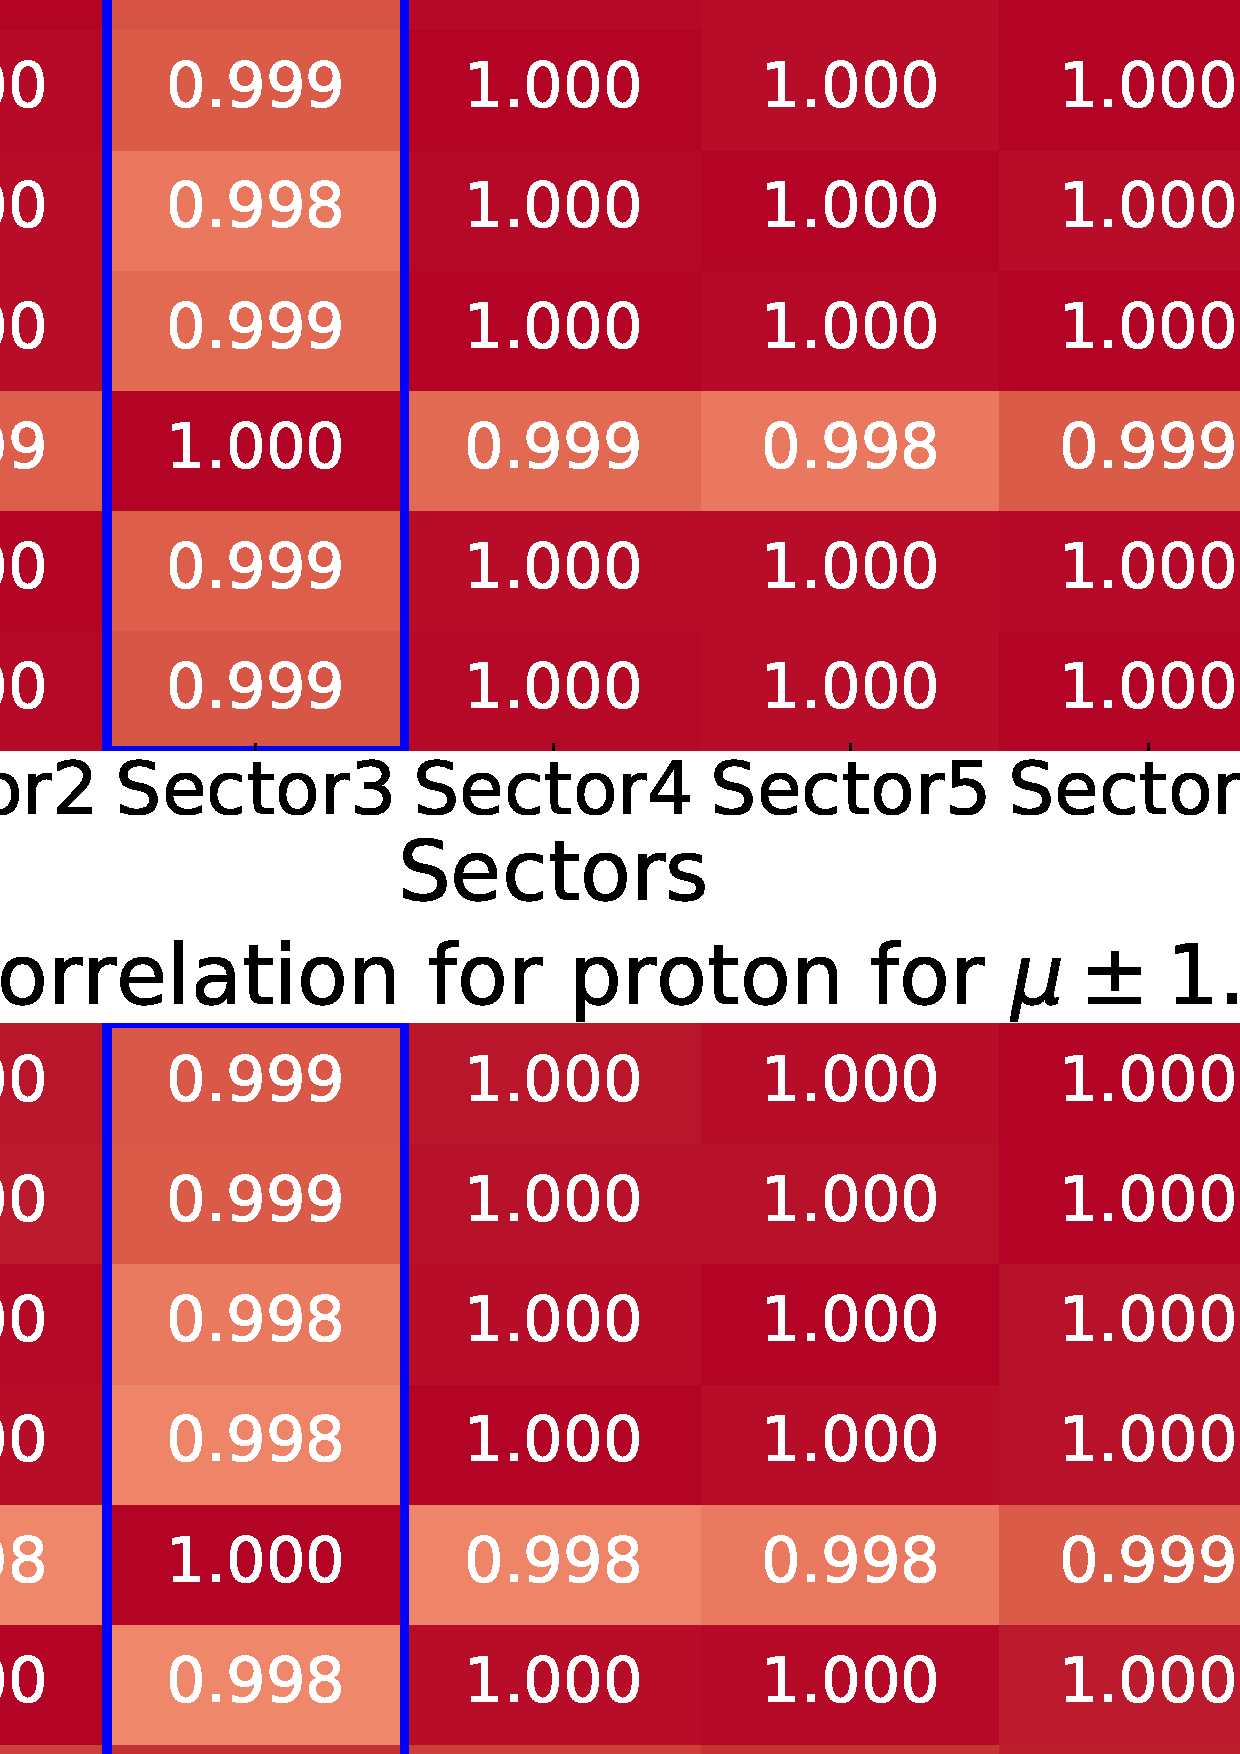
\includegraphics[width=0.85\textwidth]{images/pearson_1.png}%
    \caption{The Pearson coefficient (cf. equation \ref{pearson_coef}) calculated in order to check the possible difference in the shapes of the cross sections distributions measured in HADES detection system with the use of individual detection sectors. Example for proton distributions obtained when the width of identification cut was of 1.0 sigma (left panel) and 1.8 sigma (right panel) (For description of the width of the calibration cuts please, refer to section \ref{PID}).
    The values of coefficient for all combinations of sector results are equal to  1 what indicated that their linear correlation is maximal and discrepancies 
    in the shapes of the distributions do not exists.}
    \label{pearson_proton}
\end{figure}

In this way it was proven that the individual sector do not influence the shapes of the measured distributions. Unfortunately  
the variation in the values of cross sections obtained for individual sectors has been realized. 

The differences among values of cross sections provided by individual sectors are quantified in following way:

The ratio $R_i$ of the value of cross-section $\sigma_i$  measured in sector $i$
to the average of cross section of measured in all sectors ($j$ = 6) is given with the formula:

\begin{equation}
\label{ratio_R}
R_i = \frac{\sigma_i}{\sum_{j=1}^{6} \sigma_j /6}    
\end{equation}

whereas the error $\epsilon_i$ of this ratio is calculated as: 

\begin{equation}
\label{ratio_R_error}
\epsilon_i = \frac{5}{\sqrt{6 n_i}}
\end{equation}

It is shown in fig \ref{ratio_pos} and \ref{ratio_neg}  
the most significant differences in the absolute values of cross section in comparison to the average values are observed for sector 3 (for positively charged particles) and for sector 6 (for $\pi^{-}$).

\begin{figure}
    \centering
    \includegraphics[width=0.85\textwidth]{images/ratio_positive.png}%
    \caption{The example of the ratio $R$ given by the formula \ref{ratio_R} calculated for cross section distributions obtained for individual sectors at four selected emission angles. Here the summary cross sections for all positive particles is  taken into account. The most significant deviation of the cross section is visible for sector 3.}
    \label{ratio_pos}
\end{figure}

\begin{figure}
    \centering
    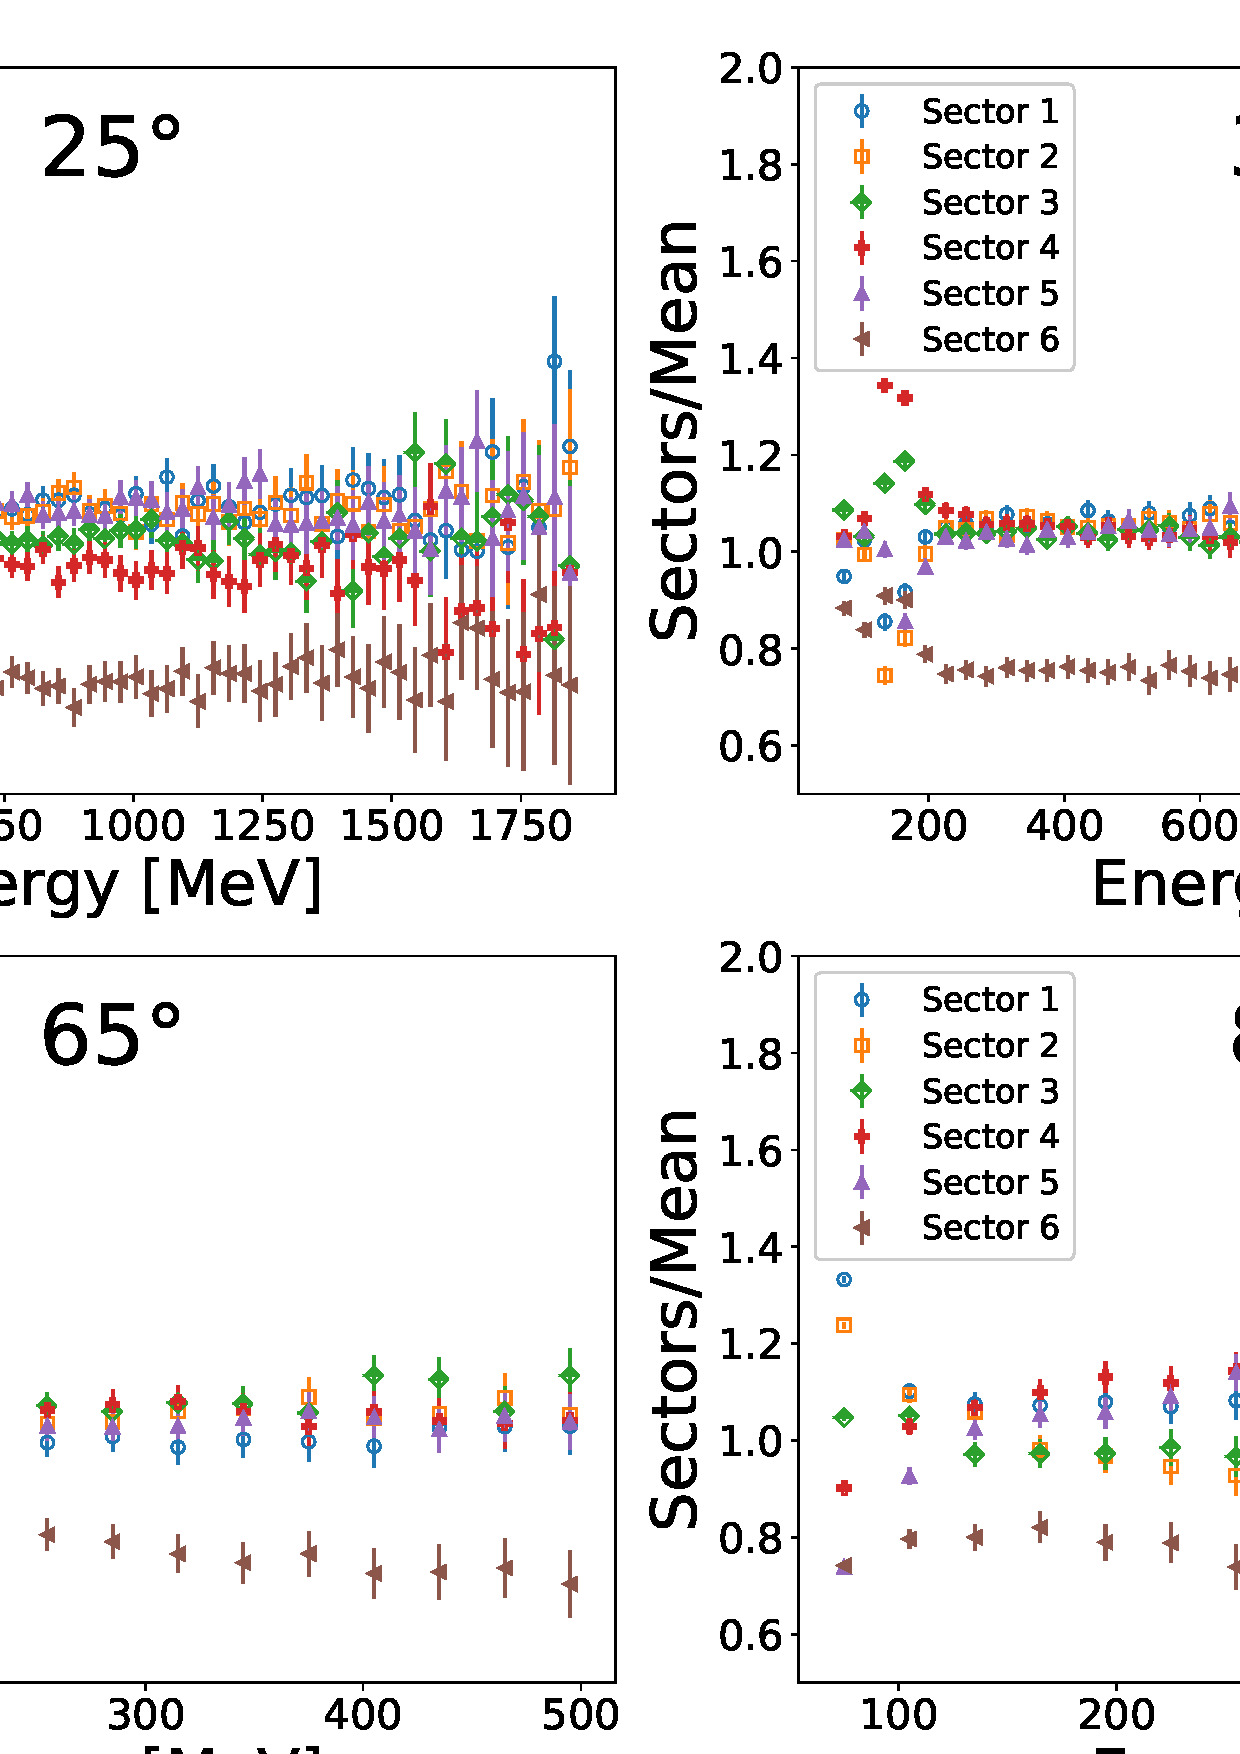
\includegraphics[width=0.85\textwidth]{images/ratio_negative.png}%
    \caption{The example of the ratio $R$ given by the formula \ref{ratio_R} calculated for $\pi^{-}$ production cross section for individual sectors at four selected emission angles. The most significant deviation of the cross section is visible for sector 6.}
    \label{ratio_neg}
\end{figure}

In order to estimate the component of cross section uncertainty (in percentage) due to variation in results of the individual sectors ($\sigma_{sect}$) the following formula has been used: 

\begin{equation}
\label{err_cs_sect}
\sigma_{sect} = (100/6) (\frac{\sigma_i - \sigma_{mean}}{\sigma_{mean}})    
\end{equation}
 
where $\sigma_{mean}$ is the average cross section among the sectors for the given particle, emission angle and the energy bin. 

The examples of $\sigma_{sect}$ are shown in 
\ref{error_cs_proton} and \ref{error_cs_pim}. 

\begin{figure}
    \centering
    \includegraphics[width=0.85\textwidth]{err_cs_proton_1.png}%
    \caption{The example of the distribution of the uncertainty $\sigma_{sect}$ resulting from the deviation of the results for sector 3 and sector 6.
    $\sigma_{sect}$ is calculated according to formula \ref{err_cs_sect} for protons detected at four selected angles.}
    \label{error_cs_proton}
\end{figure}
 
\begin{figure}
    \centering
    \includegraphics[width=0.85\textwidth]{err_cs_pim_1.png}%
    \caption{The example of the distribution of the uncertainty $\sigma_{sect}$ resulting from the deviation of the results for sector 3 and sector 6.
    $\sigma_{sect}$ is calculated according to formula \ref{err_cs_sect} for $\pi^{-}$ detected at four selected angles.}
    \label{error_cs_pim}
\end{figure} 

Considering the deviations in the magnitude of the results of individual sectors the error of the “whole” cross-section caused especially by sector 3 and sector 6 is not lager than 7\%. 

Uncertainties calculated in the way as explained above for each kind of detected particle, all selected emission angles and for 
each of energy bin
are considered as a component of the systematic uncertainty of the measured cross sections.
due to deviation in individual sector response.




 
%The differences among the sectors are %dependent on the kind of detected particle, %its energy and the emission angle. 

%In order to estimate the uncertainty component %due to the sector inequality 
%the standard deviation of the average of %results for individual sectors has been %calculated 
%for the selected particle, emission angle and the energy bin. 
%It takes values below 7\%.

%It is assumed that this value 
%estimates the systematic uncertainty resulting from the lack of full symmetry of the detection 
%system in the azimuthal angle of HADES. 

\section{\label{result_verification} Verification of results}

In order to verify the results obtained in present studies and gain  confidence about the applied data analysis scheme the relevant experimental results have been searched for in literature. The same cross sections as shown in this work are not available. Thus, the verification has to be based on the rare data of proton induced spallation but measured for different target masses and at different bombarding energies.  
It is allowed since the shapes of the spallation distributions 
in the energy and mass range of interest are similar.
It means that independently of the target mass and the proton beam energy the shape of resulting spectra are the same or change very slowly. 
The magnitude of cross section is both the energy and target mass dependent. It rises with the beam energy
and the mass number A of the target. 
But this rise is also moderate. Thus, taking into account theirs mass and energy dependence the comparison of the results 
for the similar target masses and similar beam energies is justified. 
Moreover, usually the compared spectra are biased with experimental errors of the similar range as the expected differences in the
cross sections.

As it is shown below the samples of double differential cross sections obtained in the current analysis are compared to the
other experimental results of this type. It is possible for all 
particle species studied in this thesis but only for limited 
energy and angular ranges where the similar data exists. 

At first the consistency check of the current and earlier analysis of HADES data is shown.

\subsection{\label{consistency_pim} Former HADES results for $\pi^{-}$}

The data collected for collision of $p+Nb$ at 3.5 GeV at HADES have been partially utilized earlier for studies 
of various reactions. Among them the inclusive pion and $\eta$ production has been examined \cite{AgakishievPionP}. 
In that analysis the transverse momentum distributions $dN/p_{\bot}$ 
of $\pi^{-}$ has been derived. 
This permits to perform the partial comparison of the results obtained in this thesis with the former HADES results derived from the same data but with completely different methodology. For this aim the transverse 
momenta $p_{\bot}$ of $\pi^{-}$ resulting from this analysis have been calculated.

Fig. \ref{Comp_HADES_pt1} shows the comparison of the $p_{\bot}$ distributions obtained in the former and in the current analysis. 
Both $p_{\bot}$ distributions are integrated over rapidity 
range of 0.2 $<$ $y_{lab}$ $<$ 1.8.  
The good agreement between these two distributions proves that the analysis scheme applied in this thesis provides correct results.

\begin{figure}[!h]
\centering
	\includegraphics[width=0.85\textwidth] {PtPionN.eps}%
	\caption{\label{Comp_HADES_pt1} 
		The transverse momentum, $p_{\bot}$, distribution of $\pi^{-}$ for the selected rapidity of 0.2 $<$ $y_{lab}$ $<$ 1.8 measured at HADES in $p+Nb$ at 3.5 GeV proton beam energy.
		Comparison of the results of current analysis (blue triangles) with the former studies of inclusive $\eta$ and $\pi$ production performed at HADES 
		(gray rectangles) \cite{AgakishievPionP}. 
		Despite of the various analysis schemes used the results of both of them agree very well.
	}
\end{figure}

It has to be remembered that for the $\pi^{-}$ the selection cuts 
were not needed. 
Thus, agreement of the results presented here 
proves the correctness only of the analysis steps used after the PID/background selection. 

\subsection{\label{pion_data} Mid-energy pion spectra}

Double differential cross section of similar type have been 
measured in HARP-CDP experiment %\cite{HARP_CDP_Al_2012} (and references therein).
The HARP-CDP collaboration provided the proton and pion spectra for proton induced reaction on some atomic nuclei from Be to Pb 
at 4.1 GeV proton bombarding energy  \cite{HARP_CDP_Be1_2009,HARP_CDP_Be2_2009,HARP_CDP_Ta_2009,HARP_CDP_Cu_2009,HARP_CDP_C_2010,HARP_CDP_Sn_2011,HARP_CDP_Al_2012}
. 
Among them the cross section 
for $\pi^{+}$ production in $p + ^{64}Cu$ \cite{HARP_CDP_Cu_2009} and $p + ^{181}Ta$ \cite{HARP_CDP_Ta_2009} reactions can be compared with the present results. It is done in fig. \ref{Comp_HARP_pip} where 
HADES $\pi^{+}$ data collected at $\theta$ laboratory 
angles of 65$^{\circ}$ and 80$^{\circ}$ are presented together with   
HARP-CDP results. Whereas HADES data are measured at 3.5 GeV proton energy the beam energy of HARP-CDP experiment was equal to 4.1 GeV.

\begin{figure}[!h]
    \centering
	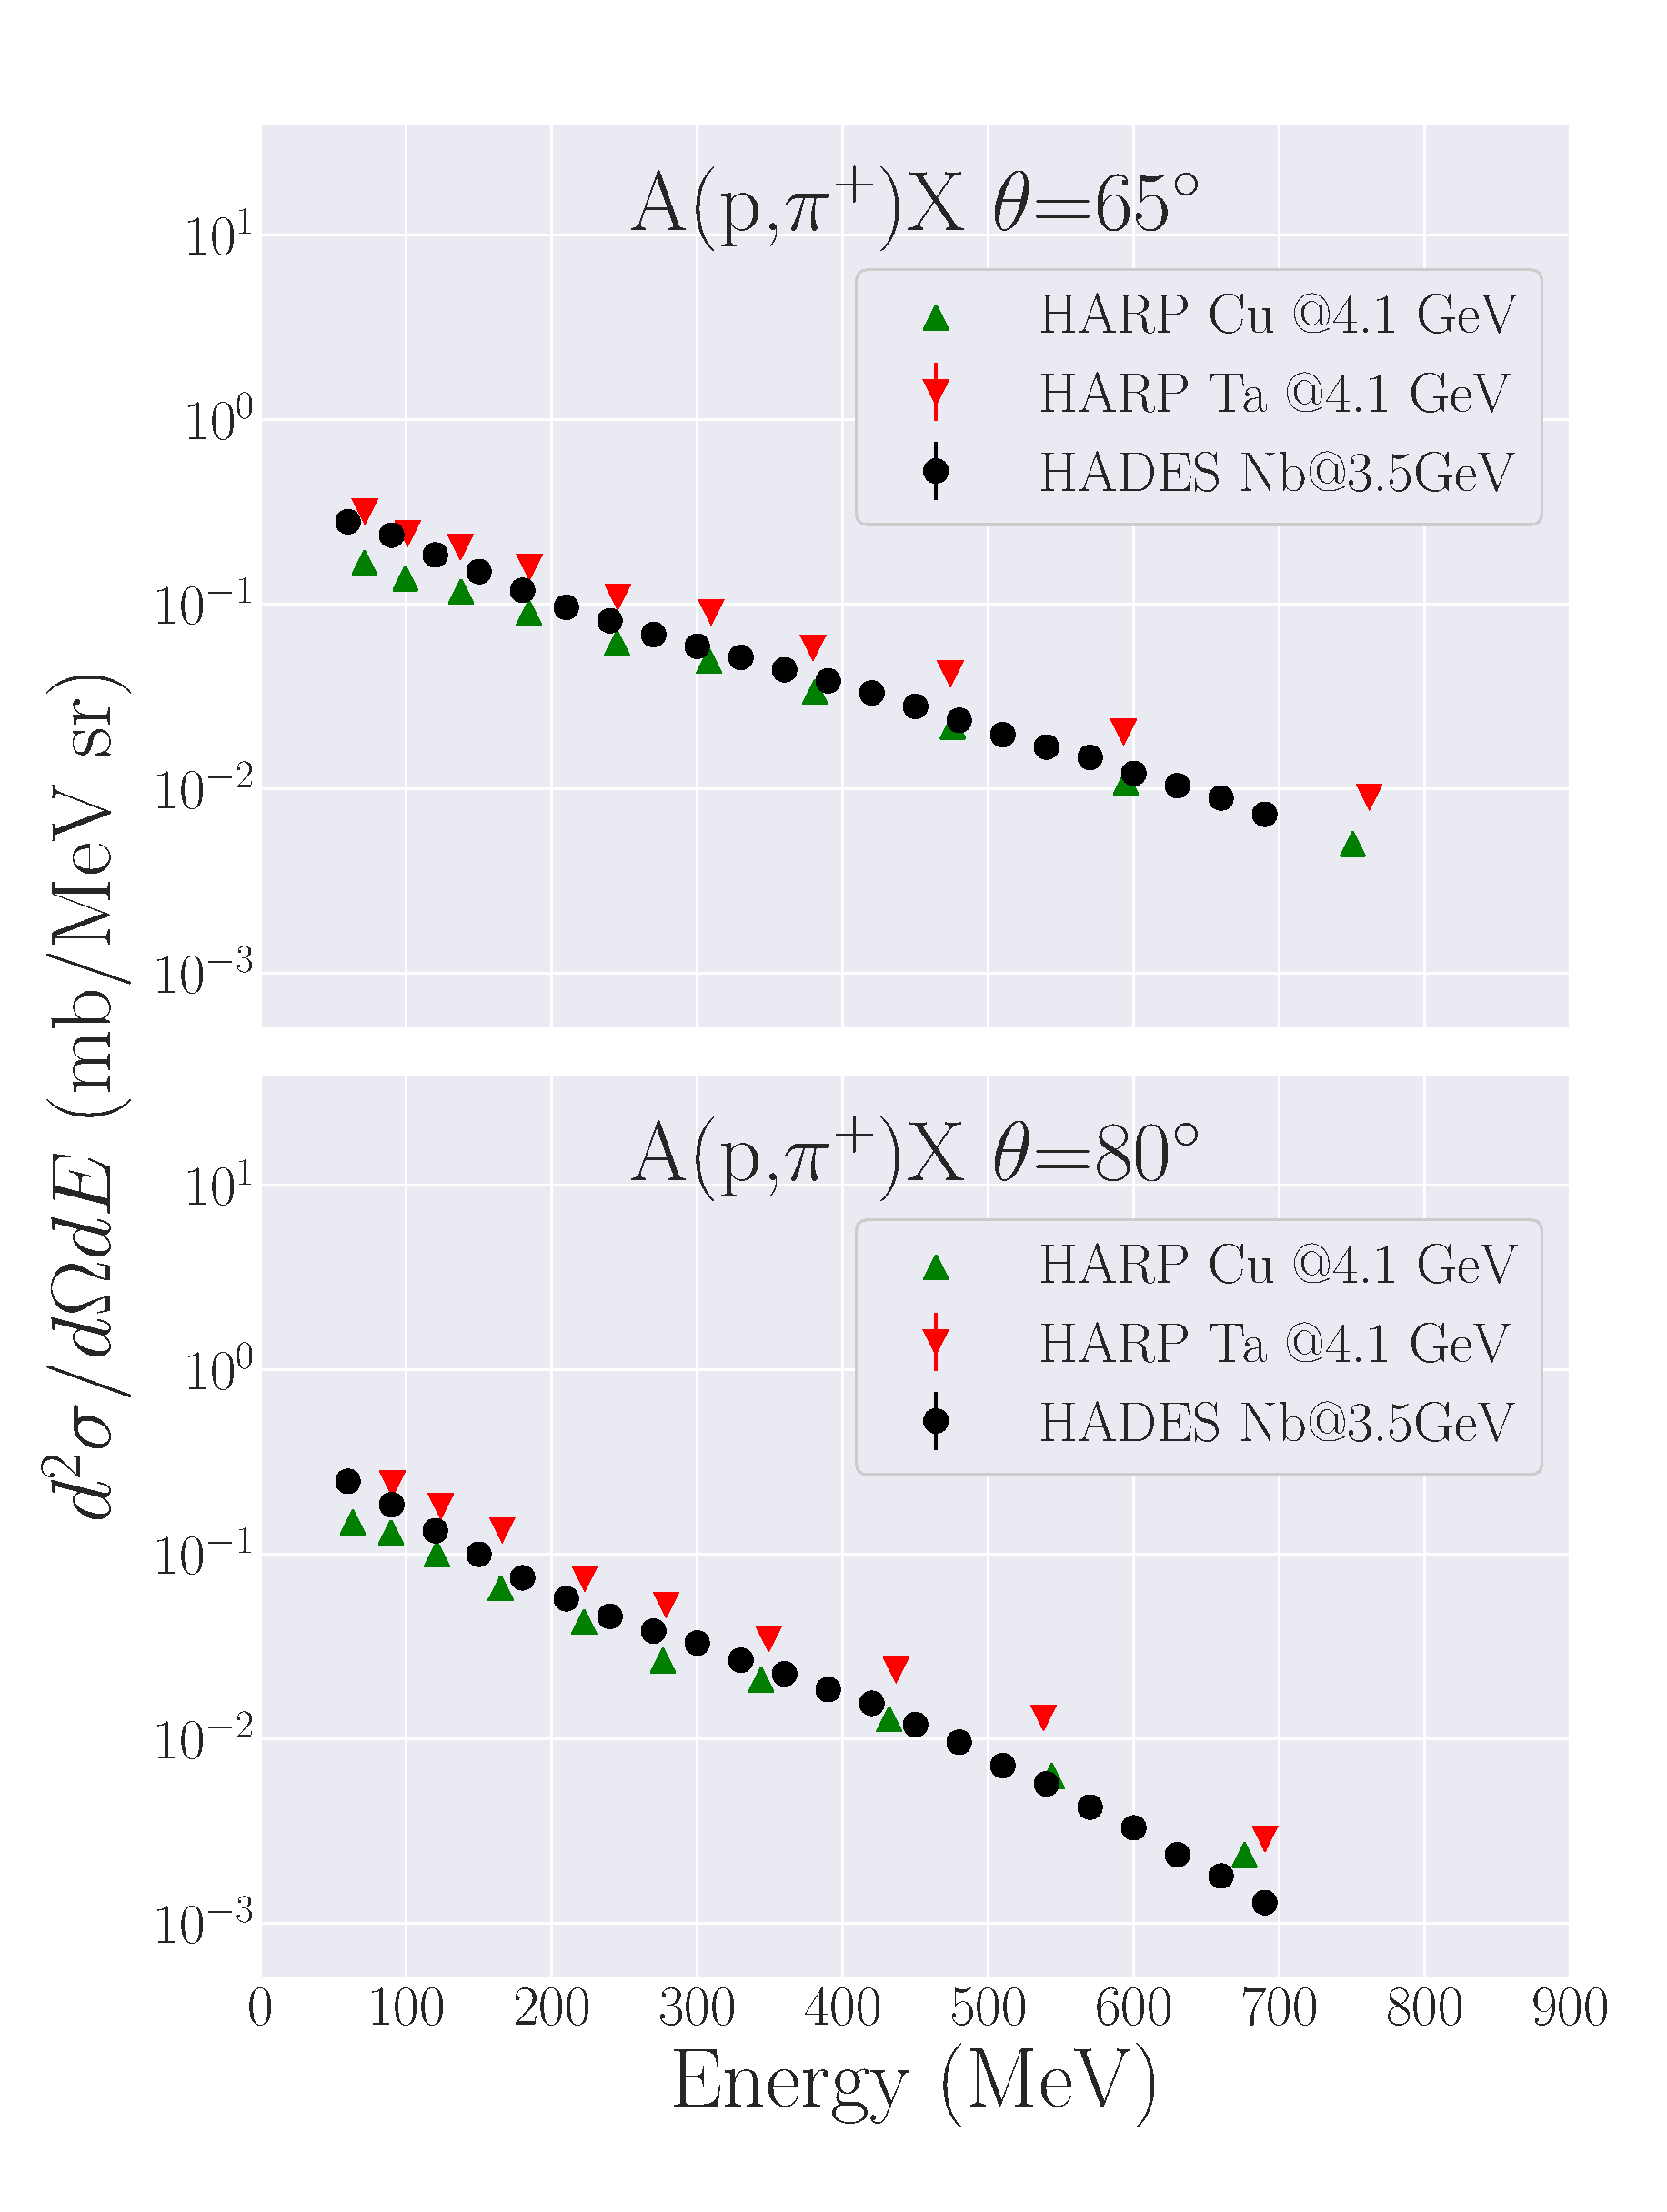
\includegraphics[width=0.65\textwidth] {PionPositive_harp_pisa.eps}%
	\caption{\label{Comp_HARP_pip} 
		Examples of double differential cross sections measured at two emission angles 
		($\theta$ = 65$^{\circ}$ - left panel, and $\theta$ = 80$^{\circ}$ - right panel) 
		at HADES for $\pi^{+}$ for $p+^{93}Nb$ @3.5 GeV (black dots). 
		They are compared to the similar results of HARP-CDP collaboration but measured for 4.1 GeV proton 
		beam impinging on $^{64}Cu$ (green triangles) \cite{HARP_CDP_Cu_2009} and $^{181}Ta$ 
		(red triangles) \cite{HARP_CDP_Ta_2009} targets.
		Taking into account the expected cross section differences due to various target masses 
		the good agreement of distributions obtained in both experiments is confirmed.
	}
\end{figure}

The shapes of energy distributions of $\pi^{+}$  
are practically the same for all three targets.
Since the proton beam energies in both experiments were similar the observed differences in the magnitudes of cross sections are practically only due to target masses. Presented spectra   
follow expected sequence of increase of the production cross section with increase of the target mass. 

This fact allows the conclusion that 
the double differential cross sections for production of $\pi^{+}$ measured at HADES agree 
well with the similar results obtained by HARP-CDP collaboration.


\subsection{\label{spal_data} Low energy spallation data}

HARP-CDP collaboration provided also the double differential cross sections for proton production in proton induced reactions. This data will be utilized here to confront the HADES result with the data available in the literature. In this respect also the
results of PISA collaboration 
\cite{fidelus2017non}  
are of interest. Data provided by PISA cover broad range of target nuclei (from C to Au) bombarded by protons of 1.2, 1.9 and 2.5 GeV energy \cite{bubak2007non,budzanowski2008competition,budzanowski2009variation,budzanowski2010comparison,fidelus2014sequential,fidelus2017non}. PISA experiment registered isotopically identified charged reaction product from $^{1}H$ to $^{12}C$ and heavier intermediate mass fragments identified only by their atomic number. 
For the aim of performed verification of the HADES results only the 
hydrogen isotopes of PISA data can be utilized.

Comparison of production cross section for $H$ isotopes measured in HADES and in PISA is given  
in fig. \ref{Comp_PISA_HARP_pdt}.  
The examples of production cross sections for 
$p$ (upper panel), $d$ (middle panel) and $t$ (lower panel) measured at HADES 
for $p+^{93}Nb$ @3.5 GeV and registered at laboratory emission angle $\theta$ = 65$^{\circ}$ are presented. The PISA results shown there as well were measured for reaction of $p+^{nat.}Ag$ @2.5 GeV  \cite{fidelus2017non} 

\begin{figure}[!h]
\centering
	\includegraphics[width=0.62\textwidth]{all_harp_pisa.eps}
	\caption{\label{Comp_PISA_HARP_pdt} 
		Examples of double differential cross sections for $p$ (upper panel), $d$ (middle panel) and $t$ 
		(lower panel) measured at HADES 
		at $\theta$ = 65$^{\circ}$ laboratory emission angle in reaction $p+^{93}Nb$ at 
		3.5 GeV beam energy.  They are confronted with the former results of spallation  
		experiment PISA \cite{fidelus2017non} for the same isotopes and detection angle. The double differential production 
		cross sections for $p$ are compared also to the results obtained in HARP-CDP experiment \cite{HARP_CDP_Cu_2009}. 
	}
\end{figure}

The HADES results for protons (upper panel) are compared also to 
the results of HARP-CDP 
registered for $p+^{64}Cu$ reaction at 4.1 GeV impinging proton energy \cite{HARP_CDP_Cu_2009}. 

The data of PISA and HARP-CDP are shown in their full available energy range wich only partially overlaps with the detection energy range of HADES experiment.

Taking into account the target mass dependence of the 
cross sections and the similar beams energies the results of HADES 
experiment are in very good agreement with those published by PISA and HARP-CDP collaborations.

The agreement of the magnitudes and the slopes of PISA, HARP-CDP and HADES distributions 
for all registered H isotopes proves the correctness of the 
data selection and analysis used in this work. 

 \ \\
 \ \\

Since the detection conditions during the $p+^{93}Nb$ run at 3.5 GeV beam energy in HADES were 
not optimized for registration of the single spectra of charged pions and hydrogen isotopes it was demanded to undertake the 
efforts in order to test if the applied analysis scheme 
including the particle identification, the background reduction and subtraction, 
the efficiency and acceptance corrections, the absolute normalization and the error 
estimation are sufficiently powerful and reliable. 
Very good agreement of the present data with those published in the literature and obtained in the experiments, 
which used completely different methods of measurements 
proves reliability of the present data processing.


 \ \\
 \ \\
 chapter 3   CORRECTED UNTIL HERE
  \ \\



\subsubsection{\label{App1} Appendix}

%\textbf{Secondary particles}:
%The problem of secondary particles is resolved by tracking %system(discussed in section 4.3 \cite{agakichiev2009HADES}). Since %tracking system track back the particle from first MDC to TOF %detectors. Secondary particles generated in random direction and %randomly from any detection system can not form track through all %four MDC modules and TOF doctors. This implies that these are %particles are already removed in track reconstruction process

\begin{figure}
	\centering
	\begin{tikzpicture}[%
		>=triangle 60,              % Nice arrows; your taste may be different
		start chain=going below,    % General flow is top-to-bottom
		node distance=8mm and 16mm, % Global setup of box spacing
		every join/.style={norm},   % Default linetype for connecting boxes
		]
		\tikzset{
			base/.style={draw, on chain, align=center, minimum height=4ex},
			proc/.style={base, rectangle, text width=6em},
			test/.style={base, diamond, text width=4em},
			term/.style={proc, rounded corners},
			% coord node style is used for placing corners of connecting lines
			coord/.style={coordinate, on chain, on grid, node distance=6mm and 25mm},
			% nmark node style is used for coordinate debugging marks
			nmark/.style={draw, cyan, circle, font={\sffamily\bfseries}},
			% -------------------------------------------------
			% Connector line styles for different parts of the diagram
			norm/.style={->, draw, lcnorm},
			free/.style={->, draw, lcfree},
			cong/.style={->, draw, lccong},
			it/.style={font={\small\itshape}}
		}
		\node [proc, densely dotted, it] (p0) {Isotropic event Generator};
		\node[term,join] (A){mult 8 or 16 events};
		\node[proc,join] (B){HGeant (Acceptance)};
		\node [proc, join] (C) {Hydra (Efficiency)};
		\node [proc, join,fill=lcfree!25] (D){Energy vs $\theta$ histogram};
		\node [proc, below=of D,fill=lcfree!25] (E){Energy vs $\theta$ histogram};
		\node[proc, join,fill=lccong!25] (F){Division 2/1};
		\node[proc, join,fill=lccong!25] (G){Efficiency + Acceptance};
% 		\node[test,join=by free](t0){Depend on mult?};
% 		\node[term] (H) {end};
		
		\node[proc,right=of A] (A1){model (e.g INCL++)};
		\node[proc,join] (B1){HGeant};
		\node [proc, join] (C1) {Hydra};
		\node[test,join=by cong](t1){M$\approxeq$HM?};
		\node [proc, fill=lcfree!25] (D1){Energy vs $\theta$ histogram};
		\node[proc,fill=lcfree!25] (E1){Energy vs $\theta$ histogram};
		\node[proc, join,fill=lccong!15] (F1){Division 5/4};
		\node[proc, join,fill=lccong!15] (G1){Efficiency + Acceptance};
% 		\node[term,join,fill=lccong!40]{end};
		\node[proc, densely dotted, it,above= of A1] (P1){Realistic generator needed};
		
		
		\node[term,right=of C1] (A2){Hades data};
		\node[proc,join] (B2){Mult(HM) histogram};
		\node[proc] (C2){Mult(M) histogram};
		\node[term,join=by free] (D2){Ratio (HM//M)};
		
		\node [coord, left=of A]  (c1)  {}; \cmark{1}
		\node [coord, right=of D]  (c2)  {}; \cmark{2}
		\node [coord, right=of G]  (c3)  {}; \cmark{3}
		\node [coord, right=of A1,xshift=-1em]  (c4)  {}; \cmark{4}
		\node [coord, right=of D1]  (c5)  {}; \cmark{5}
		\node [coord, right=of t1]  (c6)  {}; \cmark{6}
		
		\draw [*->,lcfree] (A.west) -- (c1) |- (E);
		\draw [*->,lcfree] (D.east) -- (c2) |- (F);
% 		\path (t0.south) to node [near start, xshift=1em] {$n$} (H);
% 		\draw [*->,lcnorm] (t0.south) -- (H);
% 		\path (t0.east) to node [near start, yshift=1em] {$y$} (c3);
		\draw [*->,dotted,blue, thick] (G.east) -| (c3) |- (P1);
		
		\draw [*->,lcnorm] (P1.south) -- (A1);
		\path (t1.south) to node [near start, xshift=1em] {$y$} (D1);
		\draw [*->,lcnorm] (t1.south) -- (D1);
		\path (t1.east) to node [near start, yshift=1em] {$n$} (c6);
		\draw [*->,lccong] (t1.east) -- (c6) |- node [black, near end, yshift=0.5em,xshift=4em, it]
		{Choose different models} (P1);
		
		
		
		
		\draw [*->,lcfree] (A1.east) -- (c4.south) |- (E1);
		\draw [*->,lcfree] (D1.east) -- (c5) |- (F1);
		\draw [*->, very thick,lcfree]
		(C1.south) -- ++(5mm,-5mm)  -- ++(15mm,0) 
		|- node [black, near end, yshift=-1em,xshift=-1em, it]
		{(events)} (C2.west);
		\draw [*->,  lcfree] (B2.east)   -- ++(5mm,0) |- (D2.east);
		\draw [*->,  lcnorm] (D2.south) --++(0,-50mm)  -- ++(-68mm,0) |- (t1.west);
		% \node[draw,11
		%     trapezium, 
		%      fill=blue!30,
		%     trapezium left angle = 65,
		%     trapezium right angle = 115,
		%     trapezium stretches,
		%     minimum width=2.5cm,minimum height=1cm,below= of F] (E){$dE/dx$ vs $\theta$ histogram};
		
		
		
		
		% \node[draw,
		%     trapezium,
		%     fill=blue!30,
		%     trapezium left angle = 65,
		%     trapezium right angle = 115,
		%     trapezium stretches,
		%     text width=2.5cm,minimum height=1cm,left= of D] (C){$dE/dx$ vs $\theta$ histogram};
		% \node[draw,
		%     rounded rectangle, 
		%     minimum width=2.5cm,minimum height=1cm ,below= of D, fill=red!30] (G){Efficiency};
		
		% \draw[-latex] (A) edge
		%     node[pos=0.4,fill=white,inner sep=0]{Events} (B)  (B) edge   node[pos=0.4,fill=white,inner sep=0]{Events}  (F) (C) edge  node[pos=0.4,fill=white,inner sep=0, xshift=0.75em]{1}(D);
		% \draw[-latex]    (F) edge node[pos=0.4,fill=white,inner sep=0]{Events} (E) (D) edge (G); % (E.west) edge (D.west) (D) edge (G);
		% \draw [->,MediumPurple4, thick, shorten >=1mm](A.west)-- ++(-5mm,0mm)  -- ++(0mm,-20mm) |- node[pos=0.4,fill=white,inner sep=0]{Events} (C.west);
		%\draw[-latex] (F) edge
		%   node[pos=0.4,fill=white,inner sep=0]{Events} (E) (C) edge (D) (E) edge (D) (D) edge (G);
		% \draw [|-,blue] (C.west) -- (D);
		% \draw [o->,blue] (E.south) -- (D);
	\end{tikzpicture}
	\caption{Flow chart showing the methodology for determining the efficiency of charged particles. Where multiplicity for Hades data and simulation is denoted by HM and M respectively. }
	\label{trigger_bias}
\end{figure}

\textbf{Trigger bias and efficiency}:
It is shown in figure \ref{trigger_bias} how various check are performed for estimation of efficiency these steps are performed to overcome trigger bias.
\begin{enumerate}[label=\roman*)]
    \item  To avoid influence of the trigger condition on the efficiency estimation the following analysis was performed for events containing 8 or 16 charged particles, i.e. much more abundant than the limit of 3 charged particles required by trigger condition. At first the isotropic generator was selected  in which protons are isotropically emitted with multiplicity 8 or 16 in a single event with uniform energy distribution ranging from 0 - 3500 MeV.
    \item Then these events were passed through HGeant program which simulates the generation of secondary particles in the detector and the detector acceptance.
    \item In the next step these events are passed through the HYDRA framework
which simulates the electronics behavior, track reconstruction
process and the trigger, i.e. HYDRA accepts as true events those
which correspond to at least three charged particles detected
(secondary or primary or both combined). It implies that even single
charged particle in an event activates the trigger when two or more
secondary charged particles are generated in the detector. Due to
the possibility of tracking the way of observed particles in the
detector the primary particles may be distinguished from secondary
ones. Because of this even single particle spectra of protons can be
observed with some efficiency.
    \item  After passing the events through HYDRA framework the  two dimensional histograms of energy vs $\theta$ are filled. This stage is denoted in the flowchart \ref{trigger_bias} by symbol "2". 
    \item The same histogram (energy vs $\theta$) is filled using events  generated from isotropic generator but before transferring them through HGeant and HYDRA. It is denoted by symbol "1" in flowchart  \ref{trigger_bias}.
    \item Efficiency of proton detection for isotropic emission with multiplicity(8
or 16) is calculated by dividing 2 dimensional histogram of stage
"2" by that of stage "1" in the flow chart figure \ref{trigger_bias}. Please note
that this efficiency contains also the effect of detecting system
acceptance.
    \item The projections of these two dimensional histograms (energy vs $\theta$) on
the energy axis for multiplicity 8 and 16 taken for $\theta$ range
$36^{\circ}-39^{\circ}$ are shown in fig. \ref{IsoEff}.  We can conclude
from this figure that the efficiency is dependent on multiplicity of
the charged particles in an event. This dependence is weak, however,
to obtain trustworthy result of the efficiency in the experimental
conditions one has to use the event generator with as realistic
multiplicity of particles as possible.
    \item To fulfil these conditions the INCL++ model was used to generate the
particles entering the detecting system.    The events were
simulated for conditions which are present in the p + Nb collisions
at 3.5 GeV proton beam energy. Then these events were passed through
HGeant and Hydra which simulate the detector behavior see flow chart
figure \ref{trigger_bias} for the flow of events.
%
    \item Then the comparison of distribution of  multiplicity of primary events
from  INCL++ (passed through HGeant + HYDRA) and multiplicity
distribution of data  from HADES experiment is done and results are
shown in the upper panel of figure \ref{MultINCL}. These two distributions are
normalized to the same total number of events. The ratio of the
experimental multiplicity distribution to that obtained from the
above simulation is presented in the lower panel of the figure. As
can be seen the ratio of these two distributions is close to unity
for the multiplicities in neighborhood of 3 which might be most
influenced by the trigger condition.    This may be treated as a
proof of the fact, that the event generator performed on the basis
of INCL++ is realistic.
\end{enumerate}
The above observations enable one to conclude that the trigger
condition as well as other experimental conditions can be reasonably
well simulated by INLC++ + HGeant + HYDRA frame work. This implies
that the procedure corresponding to the middle chain of figure \ref{trigger_bias} 
assures possibility of realistic estimation of the efficiency +
acceptance of the detecting system for each particle.

To calculate the efficiency following procedure was applied:
\begin{enumerate}[label=\roman*)]
    \item First the events are simulated with the INCL++ model.
    \item Then events are passed through the HGeant framework which simulates the detector acceptance.
    \item After that events are passed through HYDRA framework which simulate the trigger, electronics and track reconstruction processes.
    \item Then each particle is identified using simulation identification number (e.g proton =14).
    \item In the next step cuts are calculated with different sigma width as it was estimated for experimental data.
    \item Each of the cuts was applied on simulation data after the full analysis chain ( INCL++ + HGeant + HYDRA) to include  cuts efficiency.
    \item After applying the cuts the two dimensional histograms are filled for energy vs theta distribution and efficiency $\times$ acceptance is calculated by dividing these distribution with the distribution of INCL++ generated particles.
%    \begin{figure}[!h]
%        \centering
%        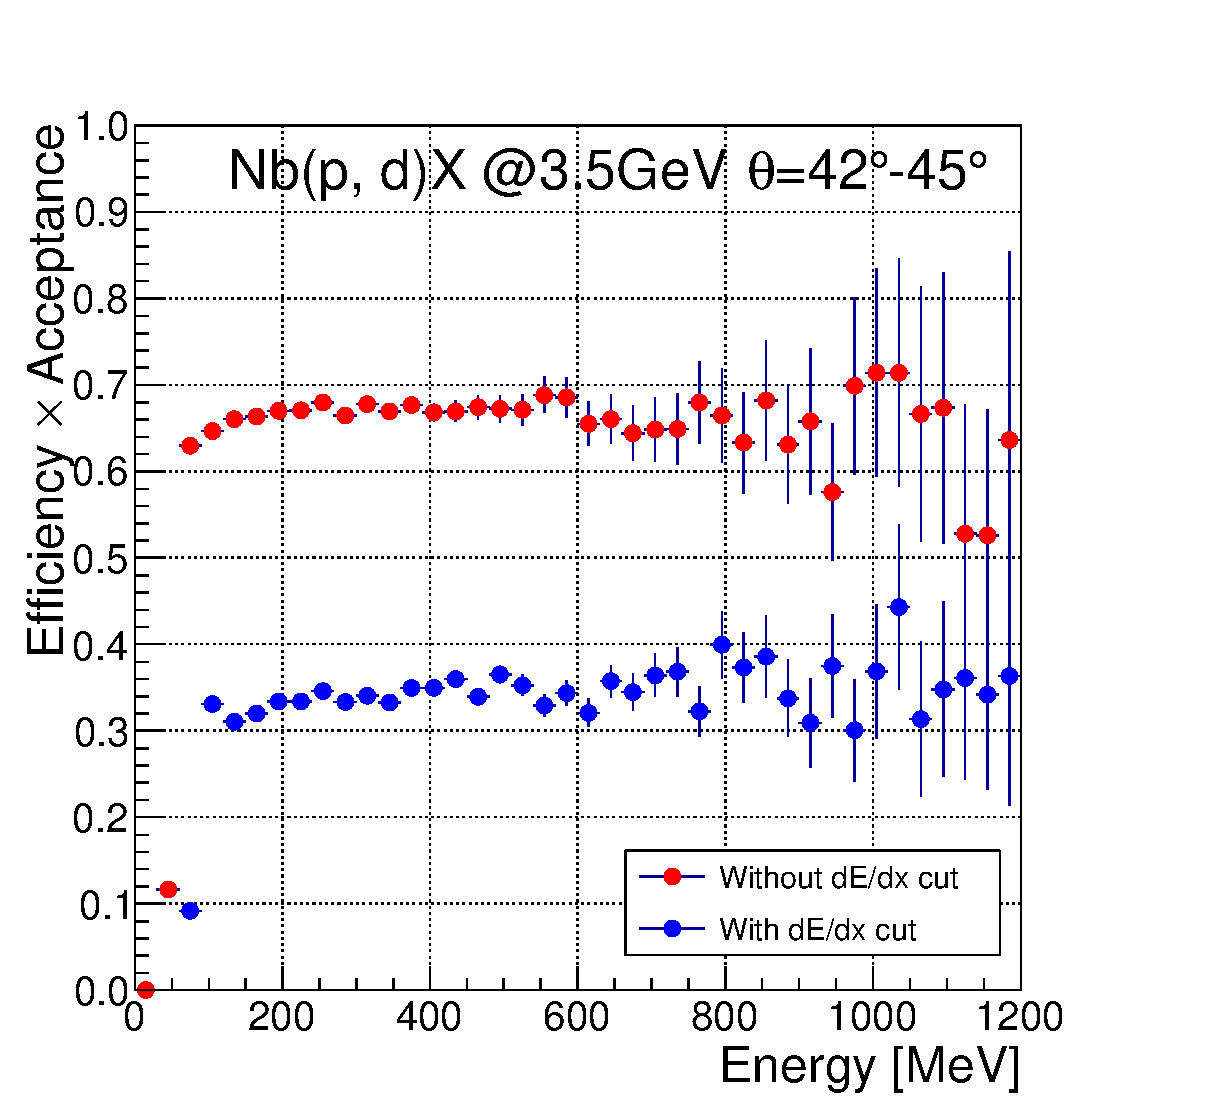
\includegraphics[width=0.95\textwidth]{DeuteronEfficiency.eps}
%        \caption{Example of HADES efficiency for registration of deuterons at $42^\circ < \theta< 45^\circ$
%        laboratory angle. The red dots represent the efficiency obtained when the PID cuts were not
%        used whereas the blue dots show the final energy dependence
%        of efficiency used for correction of absolute cross section. In
%        this case the PID cuts were applied to the ”real” distributions
%        of deuterons.}
        \label{Deuteron_effciency}
%    \end{figure}
    \item For example calculated efficiency projection for angle $42^\circ-45^\circ$ is shown in figure \ref{Deuteron_effciency}  for width =$\sigma \times 0.8$  where $\sigma$ is determined by Gaussian fitting as described for experimental data.
    
\end{enumerate}



\hspace{5cm}
%   	\includegraphics[width=0.95\textwidth]{TOF/Tofino_CUTS.png}
   	% \caption{The scatter plot of $dE/dx$ vs. $momentum$ for $p$, $d$, $t$ and $\pi^+$ registered in TOF and Tofino detectors. 
   	% The identification cuts of three widths (described above) are superimposed. 
   	%These spectra provide both the information 
   	%about "signal" of the searched for cross section as well as the background component.
    % }
   	% \label{TOF_Tofino_cut}